% !TEX program = xelatex
\documentclass[12pt,aspectratio=169]{beamer}

\makeatletter
\def\@makefnmark{}
\makeatletter

\setbeamersize{text margin left=5mm,text margin right=5mm} 

\usepackage{amsthm,amsmath,amssymb,braket,fontspec,unicode-math,fontenc}
\usepackage[absolute,overlay]{textpos}

\usetheme{moloch}
\setmainfont{SF Pro Display}
\setsansfont{SF Pro Display}
\setmathfont{Fira Math}
\setmathfont{latinmodern-math.otf}[range={frak,\bigcap,\bigcup}]

% \setbeamercolor{footnote}{fg=blue}
% \setbeamerfont{footnote}{size=\tiny}
% \setbeamerfont{title}{size=\huge}
% \setbeamerfont{subtitle}{size=\Large}
% \setbeamerfont{author}{size=\large}
% \setbeamerfont{institute}{size=\normalsize}
% \setbeamerfont{date}{size=\normalsize}
% \setbeamerfont{frametitle}{size=\large}

\usepackage[backend=bibtex,url=false,doi=false,maxcitenames=1, style=authoryear]{biblatex}
\bibliography{bib}
\AtBeginBibliography{\scriptsize}

% \newcommand{\focus}[1]{\textcolor{red}{\bf{#1}}}

% \definecolor{red}{HTML}{e03c3c}
% \definecolor{lred}{HTML}{e24a33}
% \definecolor{lblue}{HTML}{348abd}
\setbeamertemplate{bibliography item}[triangle]

% \AtBeginSection[]{
% \begin{frame}
%   \vfill
%   \centering
%   \begin{beamercolorbox}[sep=20pt,rounded=true,center]{frametitle}
%     \usebeamerfont{title}\insertsectionhead\par%
%   \end{beamercolorbox}
%   \vfill
% \end{frame}
% }
\title{
	{Holographic Entanglement in Free Fermionic Quantum Matter}
}
\subtitle{Aspects of Hierarchy and Topology in Entanglement}
\date{\today}
\author{Abhirup Mukherjee, Siddhartha Patra, Siddhartha Lal \linebreak
\alert{J. Phys. A: Math. Theor. (2024)}}
\institute{Department of Physical Sciences, IISER Kolkata Mohanpur}
\date{\today}

\begin{document}

\centering
\begin{frame}
\maketitle
\begin{textblock*}{0.25\textwidth}(12cm, 6cm)
	\centering
	\vspace*{\fill}

	
\includegraphics[width=0.45\textwidth]{figures/epqm_logo_mod.jpeg}
	\hspace*{\fill}
	
\includegraphics[width=0.45\textwidth]{figures/dps_logo.jpeg}

	\vspace*{\fill}
\end{textblock*}
\end{frame}

\section{Introduction}

\begin{frame}{Some Prerequisites}
	\begin{itemize}
		\item The system: 2D Dirac electrons\\[10pt]
		\item Entanglement of free fermions\\[10pt]
		\item Reduction of a 2D system to sum of 1D systems\\[10pt]
		\item Entanglement in topologically ordered phases\\[10pt]
		\item The holographic principle
	\end{itemize}
\end{frame}

\begin{frame}{The System: 2D Dirac Electrons}
\only<1>{
Dispersion is \alert{linear} in momentum space
\begin{center}
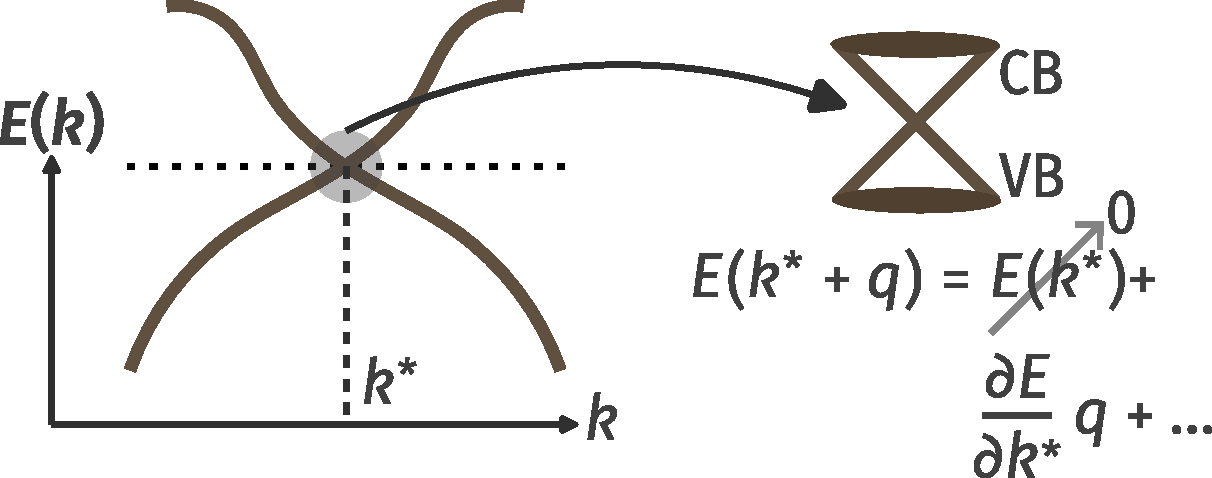
\includegraphics[width=0.8\textwidth]{figures/diracOrigin.pdf}
\end{center}
\begin{itemize}
	\item Describe the \alert{low-energy} theory near gap-closing points
	\item Emerge at boundaries of \alert{topological insulators}
\end{itemize}
}
\only<2>{
	\begin{itemize}
		\item Place on a torus (periodic boundary conditions)
		\item Insert a vector potential (flux-tuning)
	\end{itemize}

\begin{minipage}{0.4\textwidth}
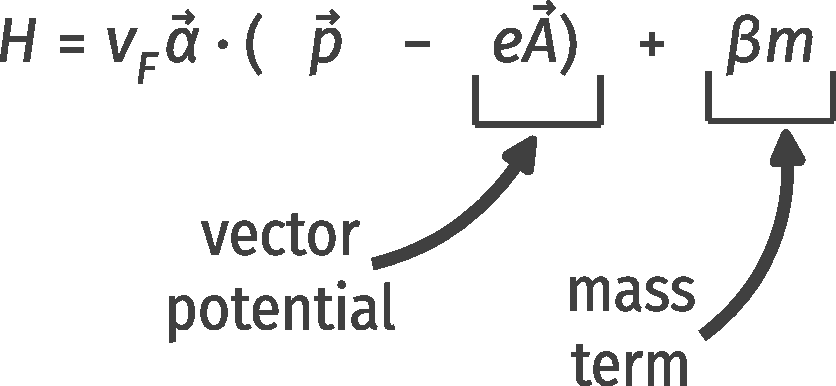
\includegraphics[width=\textwidth]{figures/diracHamiltonian.pdf}
\end{minipage}
\hspace*{\fill}
\begin{minipage}{0.4\textwidth}
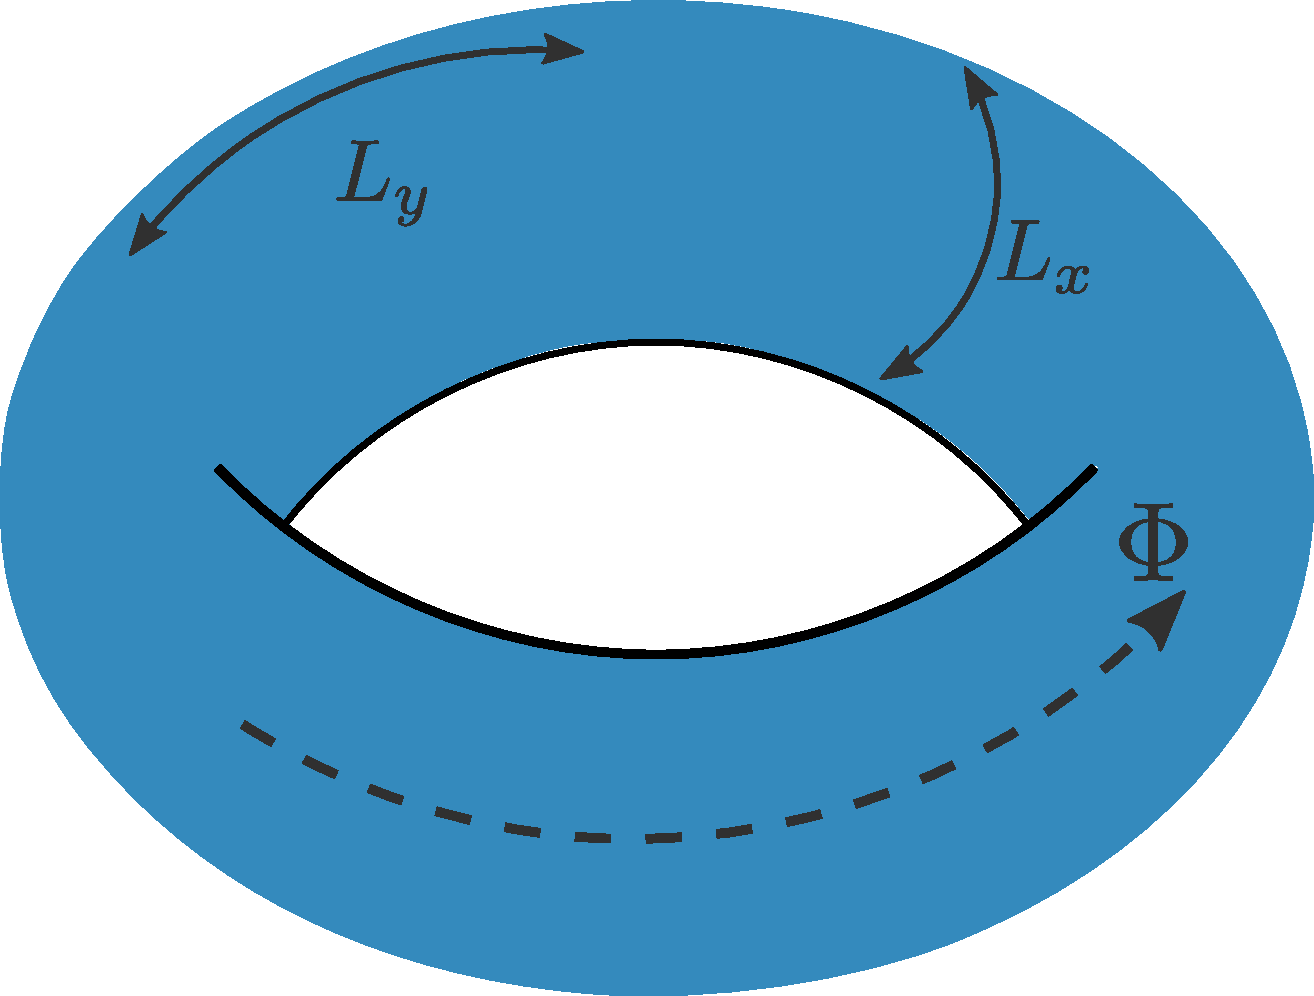
\includegraphics[width=\textwidth]{figures/torus.pdf}
\end{minipage}
}
\end{frame}

\begin{frame}{Measures of Entanglement}
	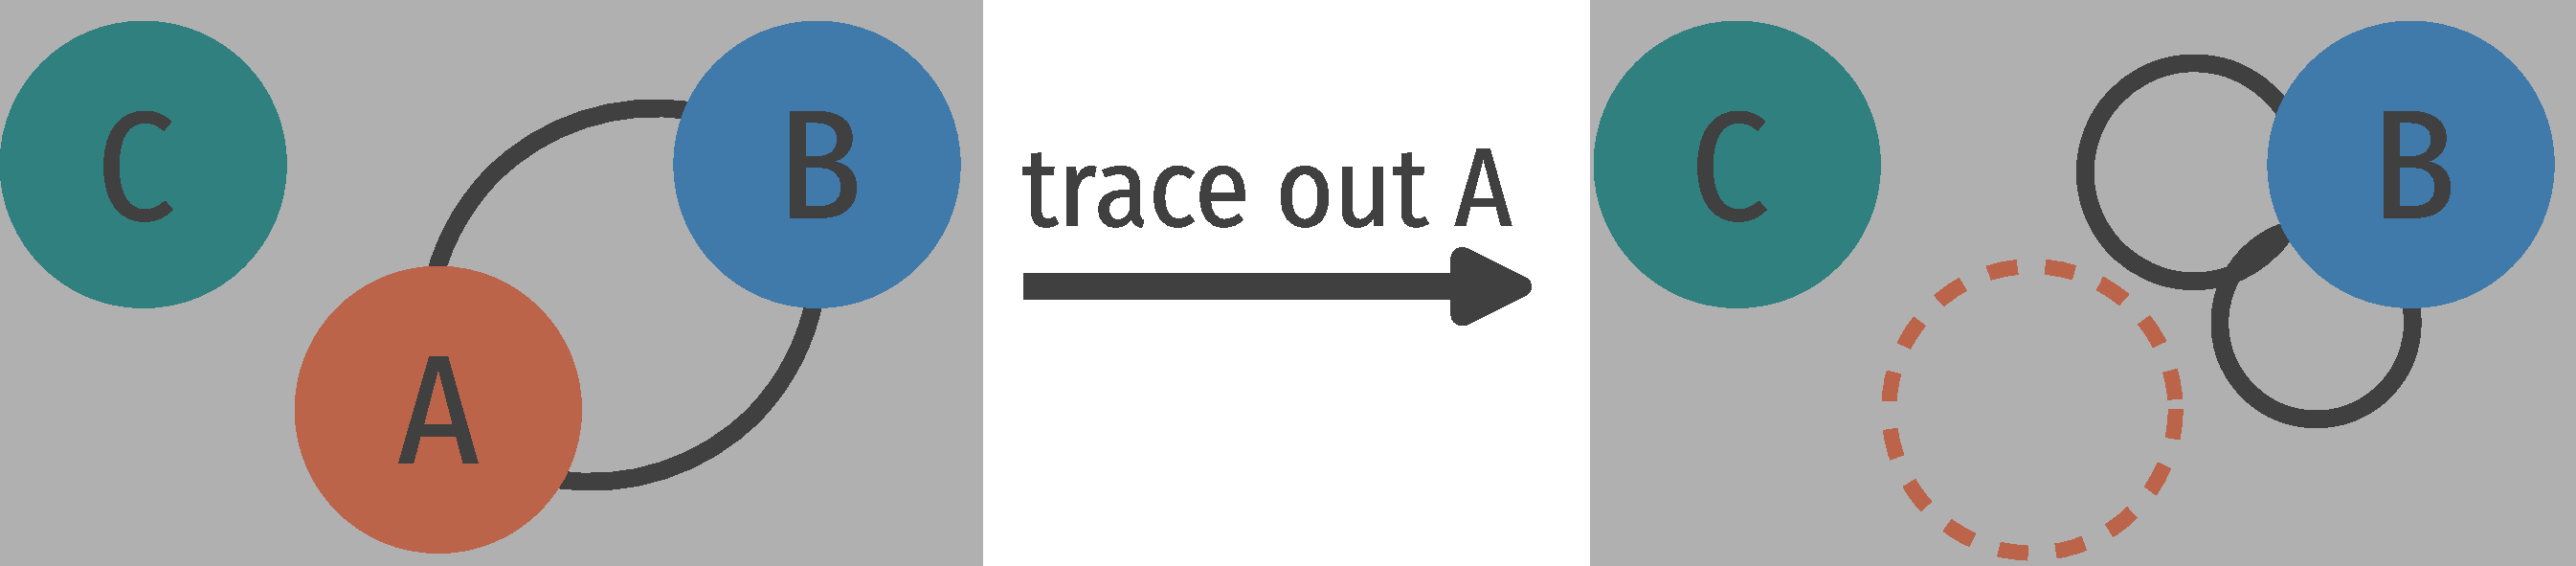
\includegraphics[width=0.9\textwidth]{figures/entanglement.pdf}
	\(\rho = \ket{\Psi}\bra{\Psi}\longrightarrow\)\alert{density matrix}\\[10pt]
	\(\rho_A = \) partial trace over system A
	\(\longrightarrow\) \alert{reduced DM}\\[10pt]
	\begin{itemize}
		\item \(S(A) = -\text{Tr}\left[\rho_A \log \rho_A\right] \longrightarrow\) \alert{entanglement entropy} of A\\[10pt]
		\item \(I(A:B) = S(A) + S(B) - S(A \cup B) \longrightarrow\) \alert{mutual information} between \(A\) and \(B\)\\[10pt]
		\item quantifies amount of \alert{information shared} between subsystems
	\end{itemize}
\end{frame}

\begin{frame}{Entanglement of Free Fermions}
\only<1>{
	Diagonal in \(k-\)space : \(H = i\overline\psi\left(\gamma_\mu\partial_\mu + m\right)\psi\)
	\begin{itemize}
		\item \alert{Vanishing} entanglement in momentum space\\[10pt]
		\item Off-diagonal in \(r-\)space \(\mathbf\longrightarrow\) \alert{Fluctuations} exist in real space\\[10pt]
		\item Leads to entanglement in real space
	\end{itemize}
	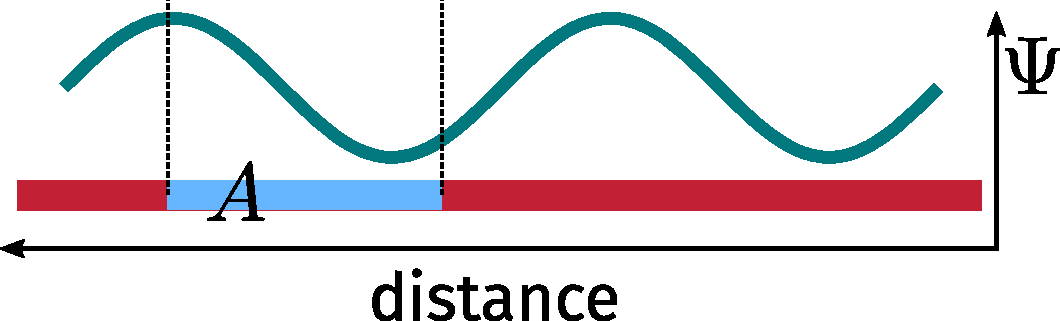
\includegraphics[width=0.6\textwidth]{figures/nonlocal.pdf}
}
\only<2>{
	Some existing results on fermionic entanglement:\\[10pt]
\begin{itemize}
	\item massless fermions in \(d-\)dimensions: \(~ ~ ~ ~ L^{d-1}\log L\)\\[20pt]
	\item massive fermions in \(1-\)dimension: \(~ ~ ~ \frac{1}{3}\log \left(L/\epsilon\right) - \frac{1}{6}\left( mL \log mL \right)^2 \)\\[20pt]
\end{itemize}
\[(\epsilon = \text{short-distance cutoff},\quad m = \text{mass gap in the spectrum})\]
\footcite{calabrese2004,Casini_2005,gioev2006,wolf_area_2006,li_scaling_2006,Casini_2009}
}
\end{frame}

\begin{frame}{Reduction of 2D System into Sum of 1D Systems}
\footcite{chung_2000,Arias_2015,Chen_2017,Murciano_2020}
\only<1>{
	In presence of flux: ~ \(\mathcal{L} = \int dx dy ~ \overline\Psi(x) \left(i\gamma_\mu + eA_\mu\right)\partial_\mu \Psi(x)\)\\[10pt]
	\begin{itemize}
		\item PBC along \(\vec x\): ~ \(\Psi(x) = \sum_{n=-\infty}^\infty e^{i x k_x^n}\Psi(k_x^n),\quad k_x^n = \frac{2\pi n }{L_x},~ ~ n \in \mathbb{Z} \)\\[10pt]
		\item Lagrangian decouples: ~ \(\mathcal{L}=\sum_{n} \int dy ~ \overline\Psi_n(y) \left(i\gamma_\mu \partial_\mu - M_n\right) \Psi_n(y)\)\\[10pt]
		\item Mass of each 1D mode: ~ {\(M_n = \frac{2\pi}{L_x}|n + \phi|\)}\\
	\end{itemize}
\includegraphics[width=0.7\textwidth]{figures/dim-reduc.pdf}
}
\only<2>{
	\vspace*{-10pt}
	\begin{itemize}
		\item \(H = \sum_n H_n \implies \rho = \exp{\left(-\beta H\right)} = \otimes_n \rho_n \implies\) no entanglement in \(k_x-\)space\\[10pt]
		\item Entanglement reduces to sum over 1D modes: \(S(\left[x_1, x_2\right])  = \sum_n S_n(\left[x_1, x_2\right])\)\\[10pt]
	\end{itemize}
	\[S_n(\phi) = \underbrace{c \log \left(\alpha L_x\right)}_\text{modified area law} - \underbrace{c \log |n + \phi|}_\text{mass correction},\quad \alpha\longrightarrow \text{ cutoff dependent constant}\]
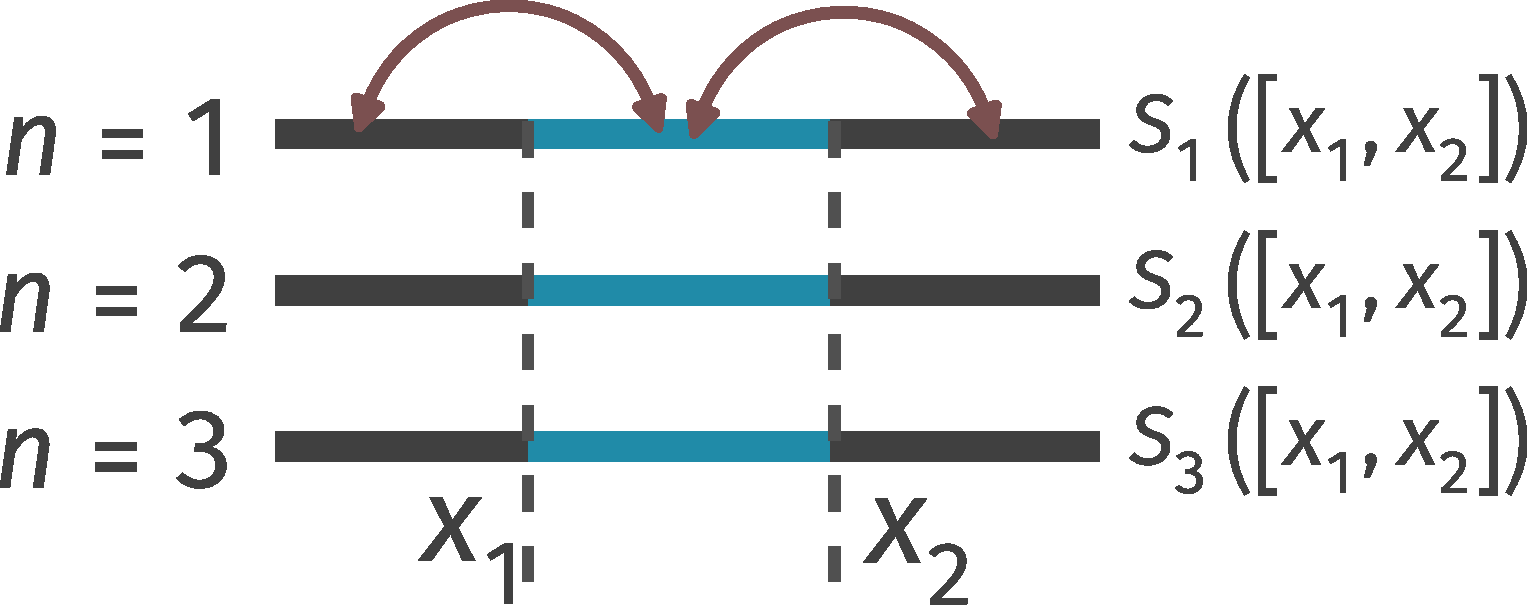
\includegraphics[width=0.5\textwidth]{figures/entanglementSum.pdf}
}
\end{frame}

\begin{frame}{Entanglement in Topologically Ordered Phases}
	\footcite{wen_1989,kitaev2006topological,Patra2022}
	\alert{Gapped quantum liquids} arising from strong inter-electron correlations\\[10pt]
	\begin{itemize}
		\item FQHE, Toric Code, Kitaev's honeycomb model, QSLs\\[10pt]
		\item robust ground-state \alert{degeneracy} on closed manifolds (for eg., torus),\\[10pt]
	\item \alert{long-ranged} entanglement: \(S(L) = \alpha L - \gamma + \mathcal{O}(1/L)\).\\[10pt]
	\end{itemize}
	\(N-\)partite information measure depends on \(\gamma\) and the Euler characteristic \(\chi\) of the manifold: \(|I_N| = \gamma \chi\).
\end{frame}

\begin{frame}{The AdS-CFT Correspondence: A Holographic Duality Relation}
	\only<1>{
	\alert{What is a duality?} 

	Different Hamiltonian/action describing the same system
	\vspace*{15pt}

	Example: Quantum-Classical Mapping

	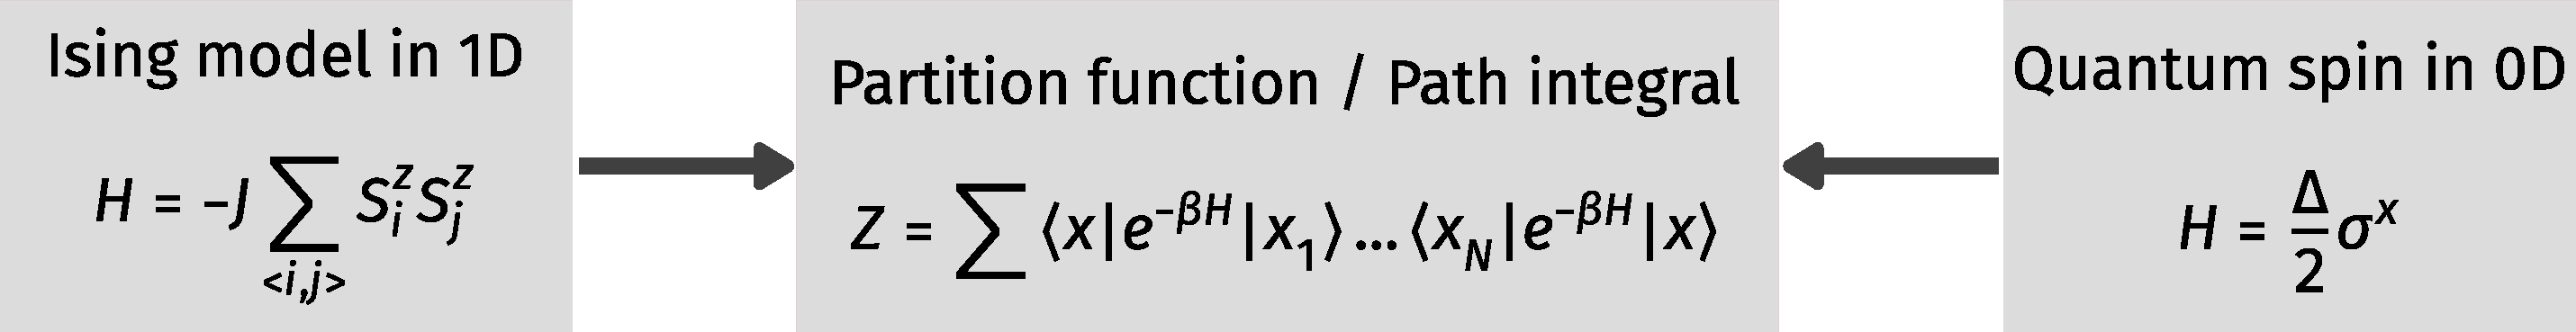
\includegraphics[width=0.9\textwidth]{figures/classical-quantum-correspondence.pdf}

	\vspace*{15pt}
	Another example: Maxwell's equations\\[5pt]
	\(\nabla\cdot{\bf E} = \nabla\cdot{\bf B} = 0, \nabla \times {\bf E} = -\frac{\partial {\bf B}}{\partial t}, \nabla \times {\bf B} = \frac{\partial {\bf E}}{\partial t}\)\\[5pt]
	\(\text{under the transformation }\quad {\bf E} \to -{\bf B}\)

}
\only<2>{
	\footcite{green2013holography,sachdev2012gaugegravity}
	\alert{What is AdS-CFT?}

	\vspace*{\fill}
	\begin{minipage}{0.45\textwidth}
	Duality between a gravity theory and a conformal field theory
	\[\underbrace{~~Z_\text{Q}~~}_\text{D dims} \sim \underbrace{\exp\left(-\mathcal{S}_\text{cl}\right)}_\text{D+1 dims}\]
	\end{minipage}
	\hspace*{\fill}
	\begin{minipage}{0.45\textwidth}
	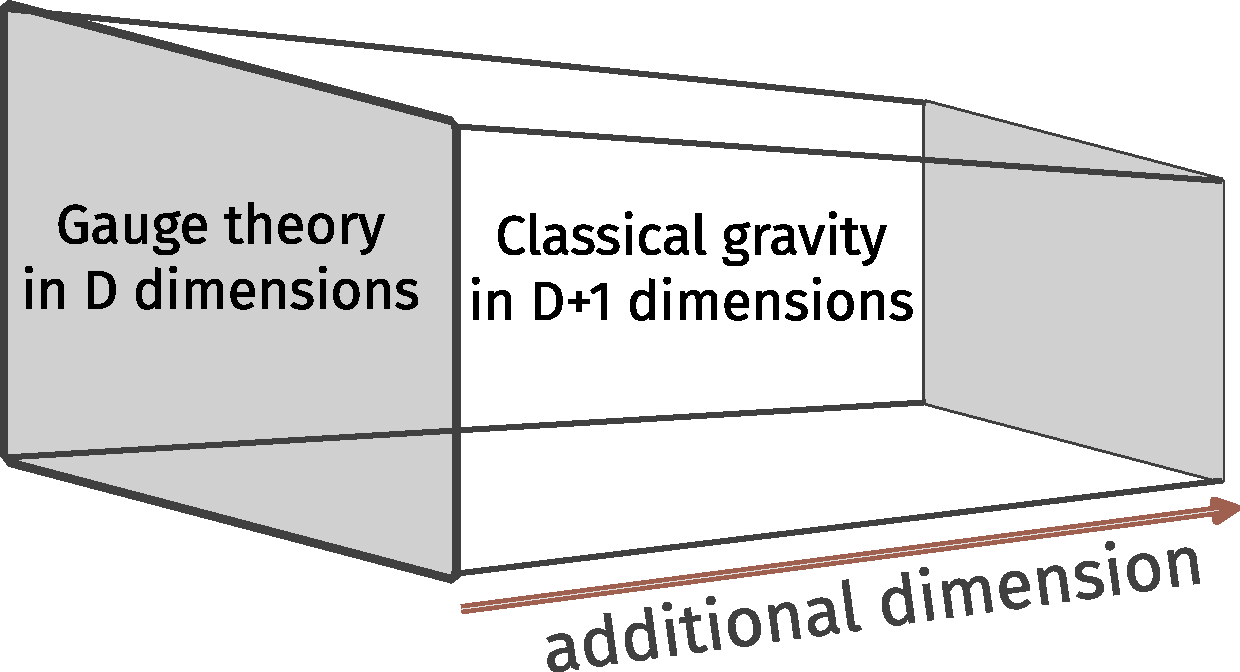
\includegraphics[width=\textwidth]{figures/AdS-CFT.pdf}
	\end{minipage}

	\vspace*{\fill}
	CFT: Remains invariant under \alert{conformal transformations}
	\[g_{\mu\nu}(x) \to \Lambda(x) g_{\mu\nu}(x)\]
}
\only<3>{
	\footcite{bekenstein1973,akhmedov_1998,alvarez_1999}
	\alert{What is holography?} \\
	Amount of information within a region is bounded by the surface area!\\[10pt]
	Entropy of a black hole: \(S_\text{BH} = \frac{k_B}{4 l_P^2} A_H\)\\[10pt]

	\vspace*{\fill}
	\alert{Physical Interpretation of the Additional Dimension}

	\begin{minipage}{0.35\textwidth}
	{\it renormalisation group} \\
	flow of\\
	boundary CFT
	\end{minipage}
	\begin{minipage}{0.55\textwidth}
	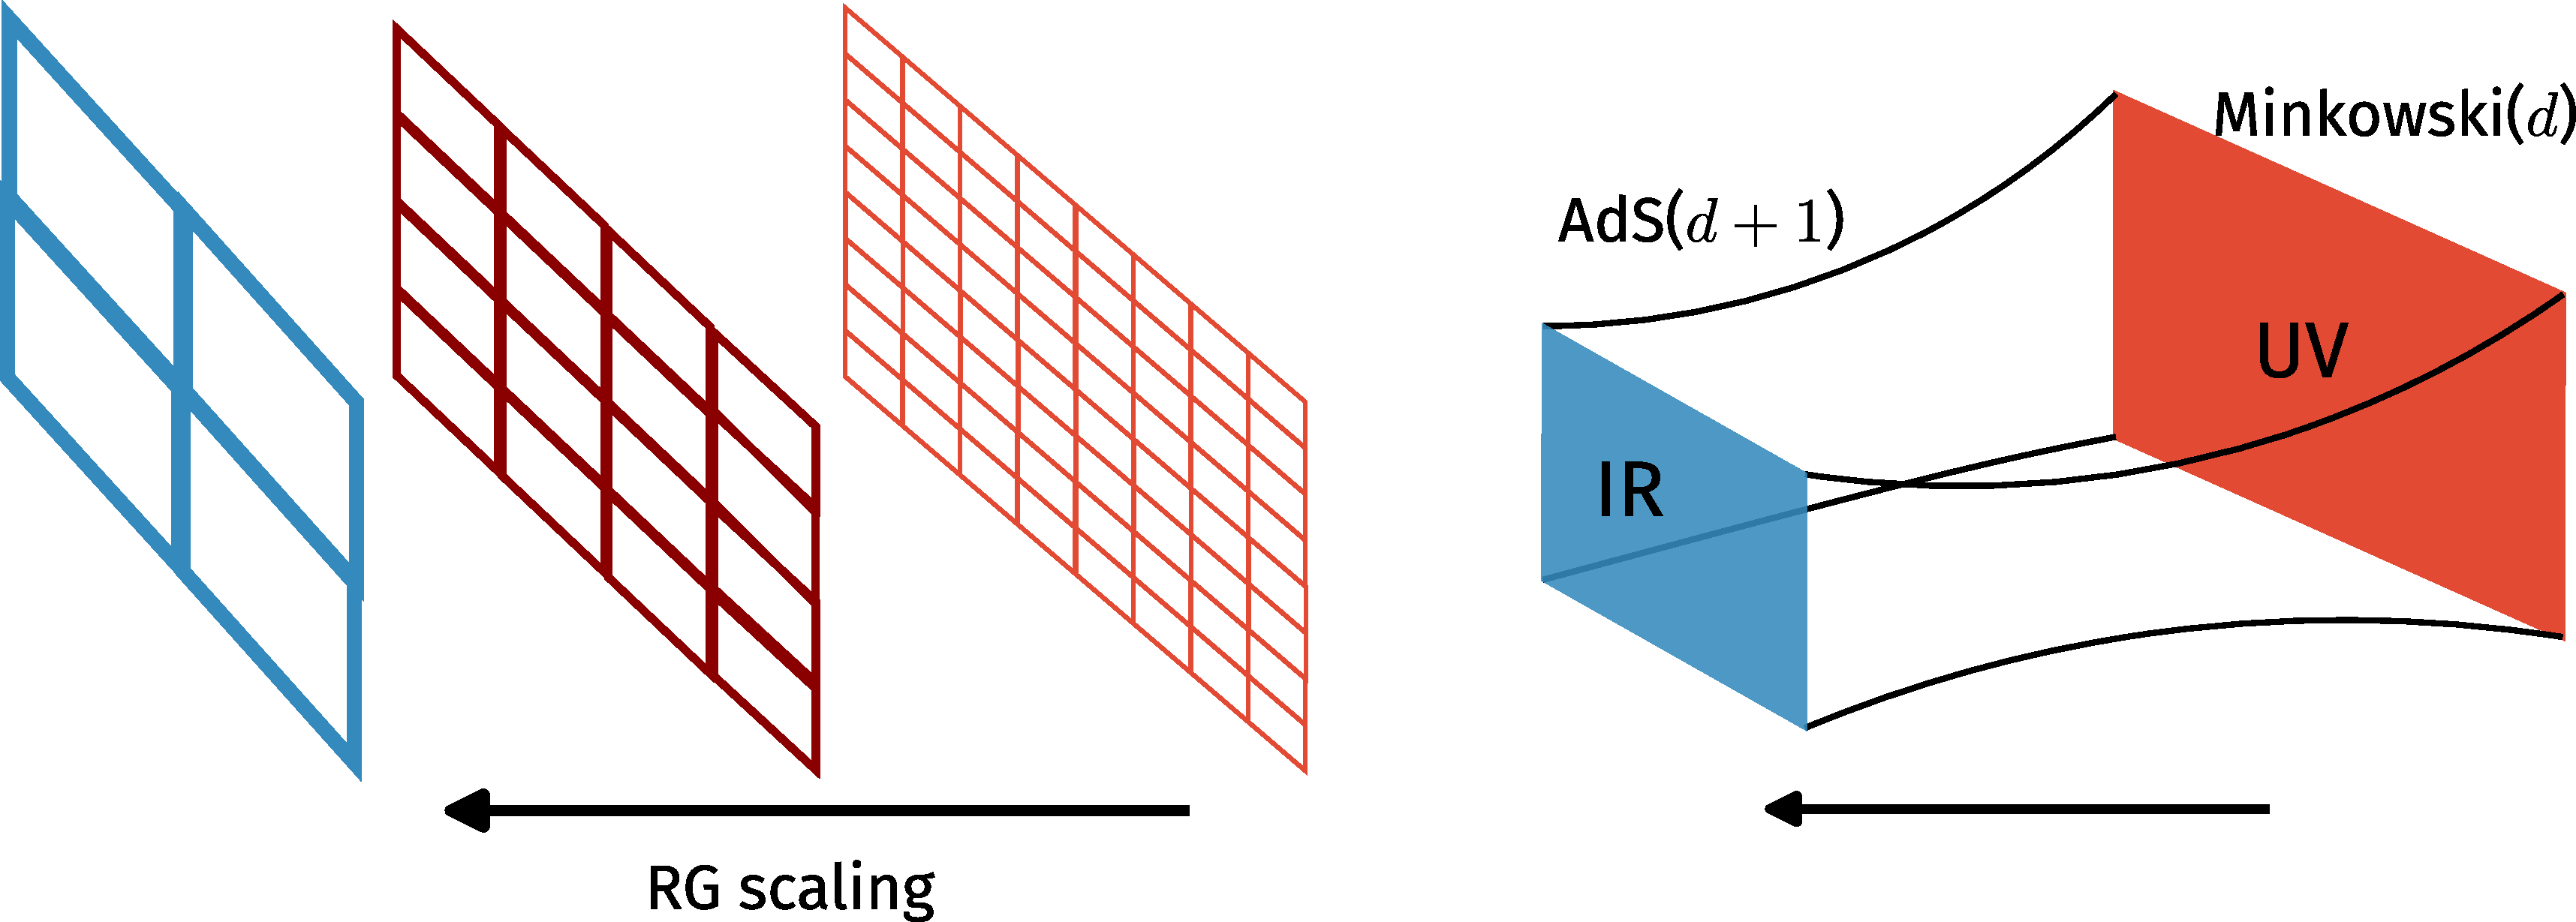
\includegraphics[width=\textwidth]{figures/holography.pdf}
	\end{minipage}
}
\end{frame}

\section{What are we going after?}

\begin{frame}{What Are We Going After?}
	\begin{itemize}
		\item Distribution of entanglement across subsystems and scales\\ (\alert{RG flow of entanglement})\\[10pt]
		\item Topological aspects of entanglement\\ (\alert{link to Fermi volume})\\[10pt]
		\item Emergent space generated by this entanglement\\ (\alert{holography})\\[10pt]
		\item Curvature and related quantities of this emergent space\\ (\alert{curvature transition})\\[10pt]
		\item Effect of boundary phase transition on the emergent space\\ (\alert{phase transition = wormhole geomtry})
	\end{itemize}

\end{frame}

\section{Entanglement Hierarchy in Mixed Momentum and Real Space}

\begin{frame}{Creating Subsystems}
	\[k_x^n = \frac{2\pi }{L_x} n,~ ~ n \in \mathbb{Z};~~~ \text{define \alert{distance}} = \Delta n = 1\]
	\alert{Simplest} choice: the entire set
	\[\text{distance} = 1 \longrightarrow n \in \left\{0,1,\ldots,N-2,N-1,N\right\} \]
	\alert{Coarser} choices: increase distance
	\[\text{distance} = 2 \longrightarrow n \in \left\{0,2,\ldots,N-4,N-2,N\right\} \]
	\[\text{distance} = 4 \longrightarrow n \in \left\{0,4,\ldots,N-8,N-4,N\right\} \]
	\centering
	\vspace*{\fill}
	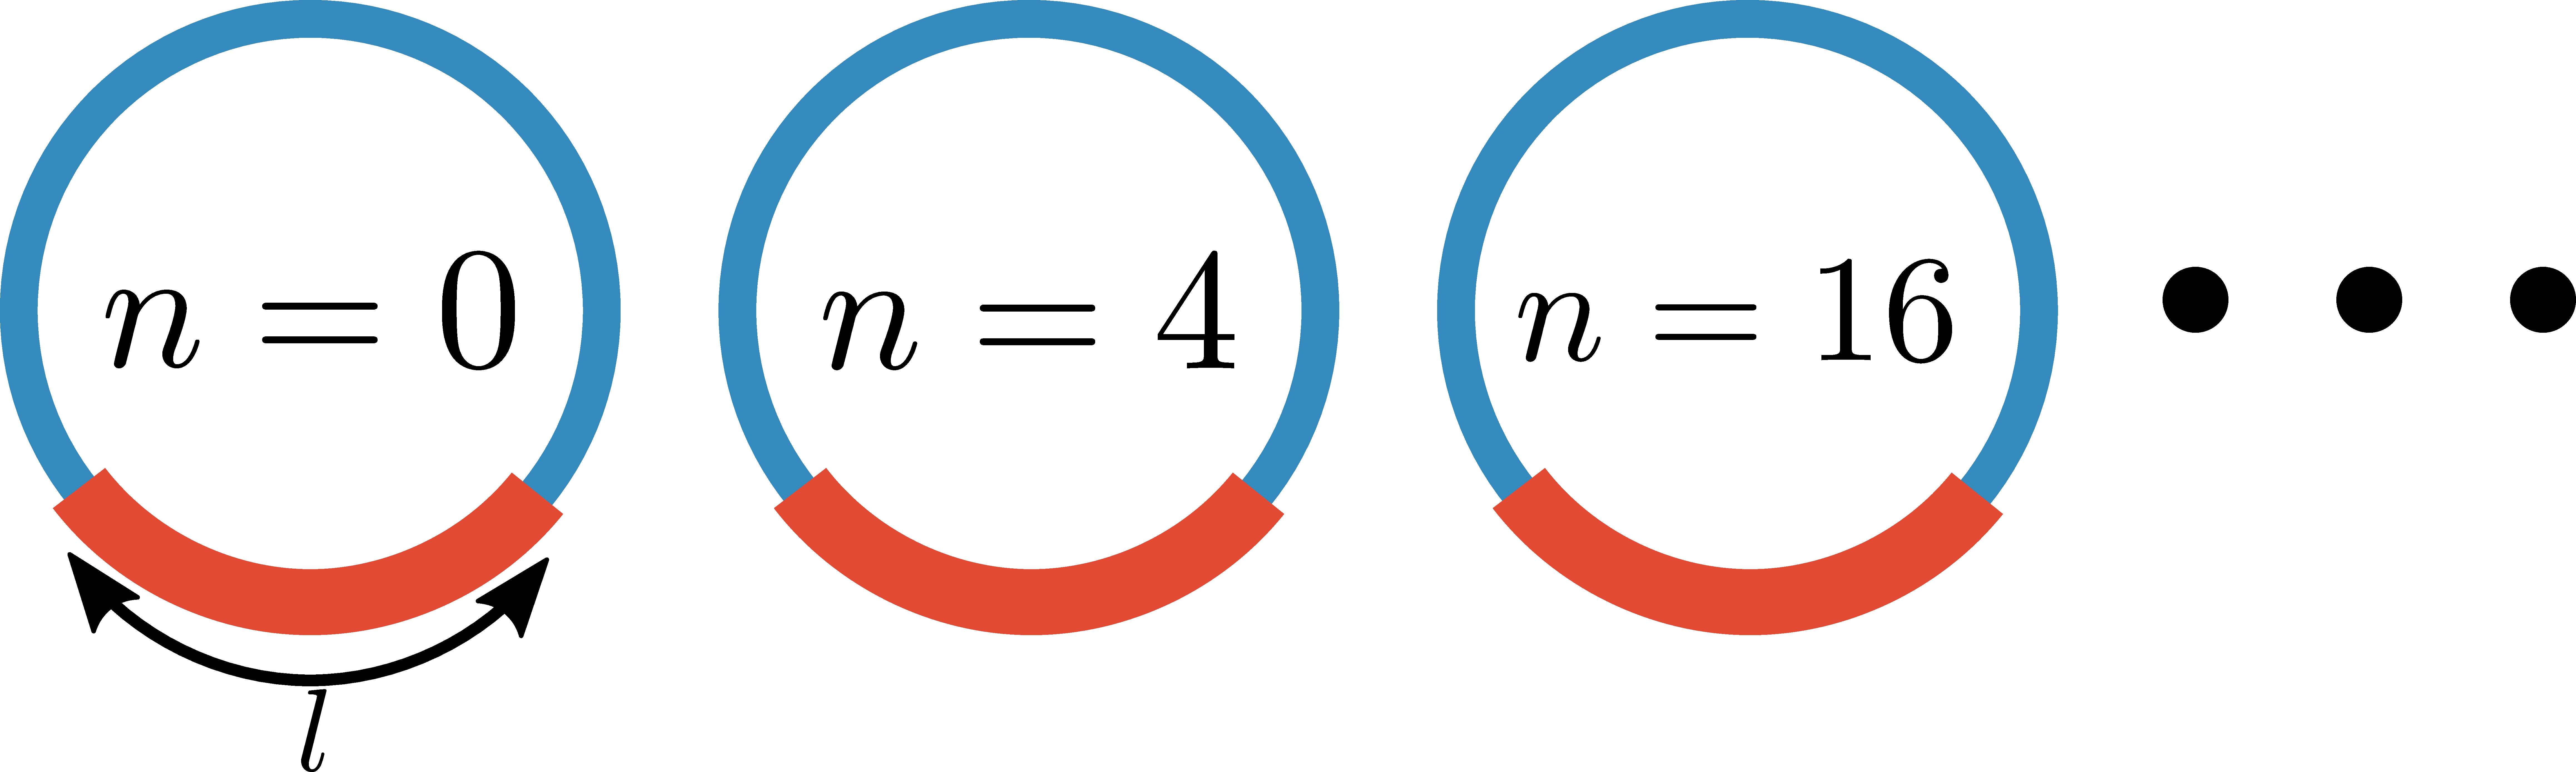
\includegraphics[width=0.4\textwidth]{figures/A_mi.pdf}
\end{frame}

\begin{frame}{Define Sequence of Subsystems}

\(~ ~ k_x^j = \frac{2\pi}{L_x}t_z(j), ~ ~ ~ t_z(j) = 2^{j^z}\);~ ~ ~sequence index: \(j = 0,1,2,\ldots\)
\[\text{strength of coarse/fine-graining:}~ ~ ~ z = \pm 1,\pm 2,\pm 3,\ldots\]
\begin{minipage}{0.48\textwidth}
\centering
\( z = 1\)\\
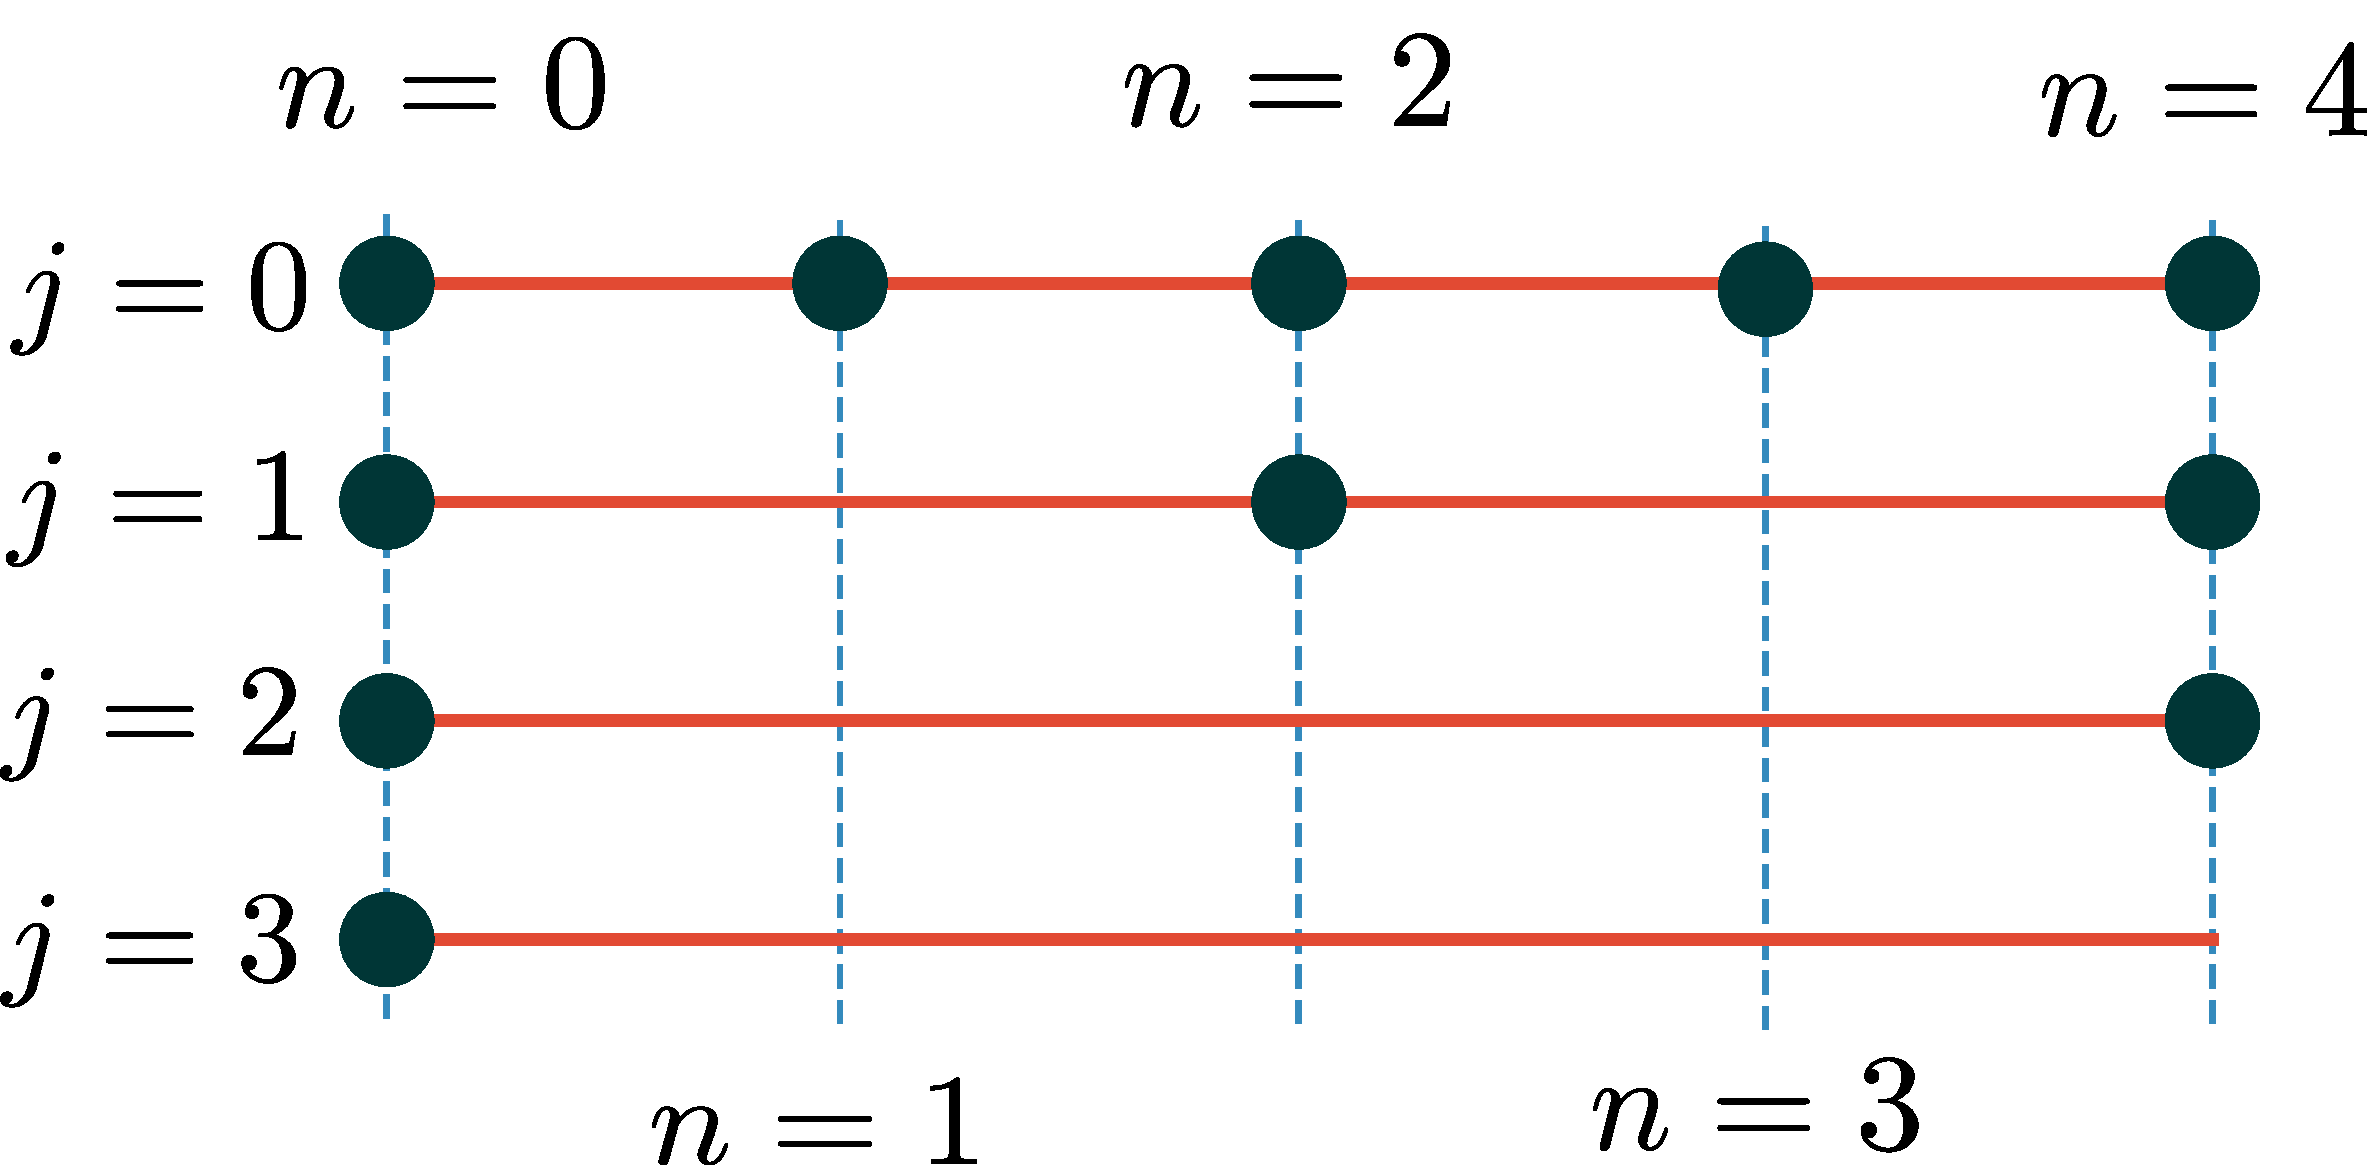
\includegraphics[width=0.99\textwidth]{./figures/coarse-graining.pdf}
\end{minipage}
\hspace*{\fill}
\begin{minipage}{0.49\textwidth}
\centering
\( z = -1\)\\
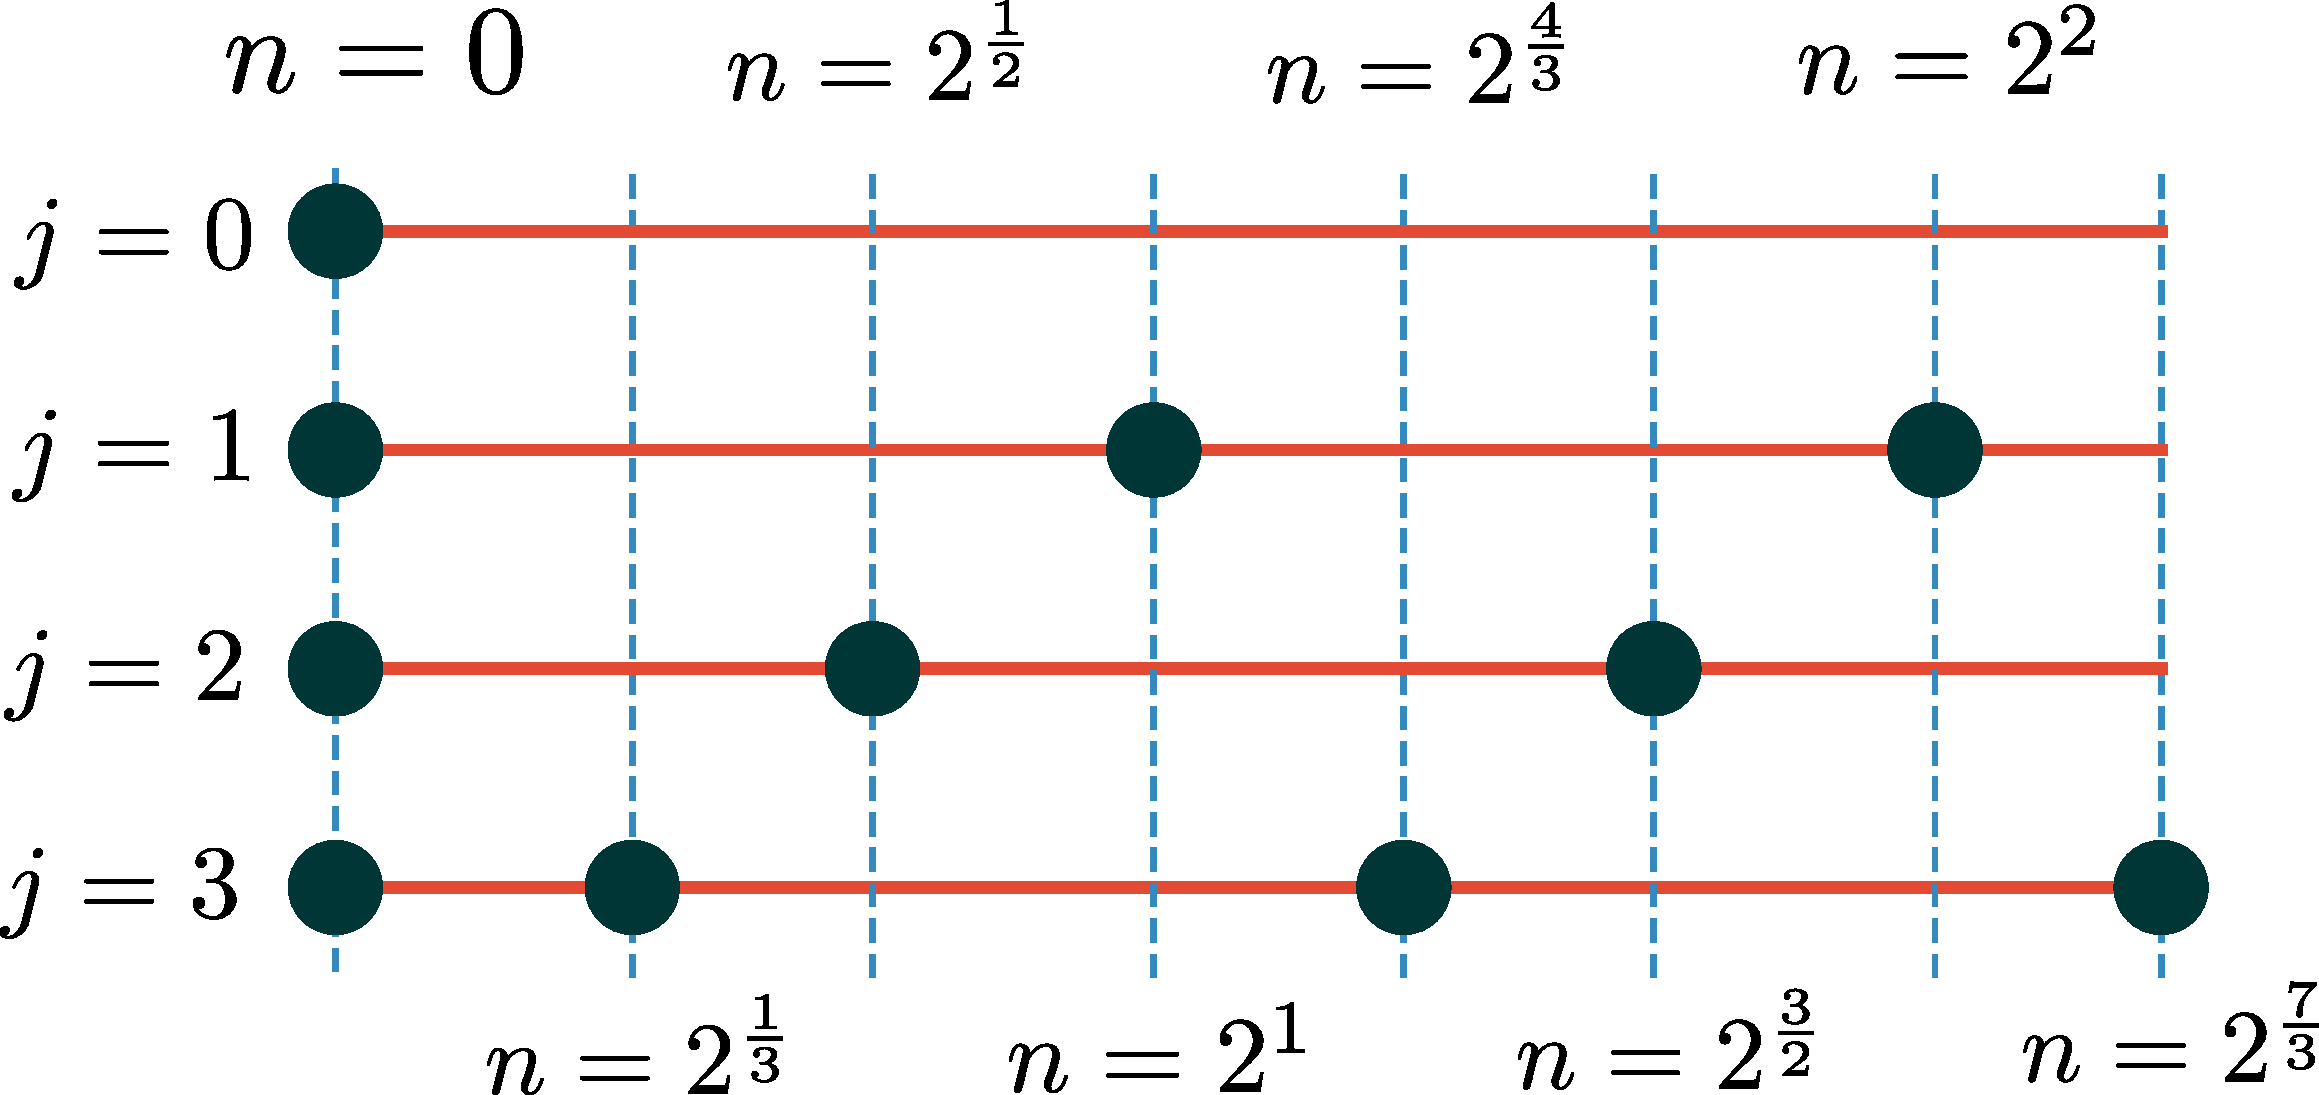
\includegraphics[width=0.99\textwidth]{./figures/fine-graining.pdf}
\end{minipage}
\end{frame}

\begin{frame}{Interpreting the Set of Transformations as an RG Flow}
	Sequence of Hamiltonians \(\leftrightarrow\) \alert{renormalisation} group flow\\[10pt]
	RG \(\rightarrow\) transformation of Hamiltonian via change of scale\\
	\[\text{Superset of all members:}~ ~ ~ \mathcal{A}_z^{(0)} = \bigcup_j \mathcal{A}_z(j)\]
	\[\text{"Super-Hamiltonian":}~ ~ ~\mathcal{H}^{(0)} = \sum_{k_x \in \mathcal{A}_z^{(0)}} \mathcal{H}\left( k_x \right)\]
	\[\text{RG equation:}~ ~ ~\mathcal{H}_z(j) = \underbrace{\mathcal{P}_z(j)}_\text{projector} ~ \mathcal{H}^{(0)} ~ \mathcal{P}_z(j)\]
\end{frame}

\begin{frame}{So What, Exactly, is Getting Renormalised?}
	Several ways to look at this\\[10pt]
	\begin{itemize}
		\item renormalisation in \alert{entanglement}: \(\Delta \log S_z(j) \sim \Delta f_z(j) \)\\[10pt]
		\item renormalisation in 1-particle \alert{spectral gap}: \(M(n,\phi) \sim |n + \phi|\)\\[10pt]
		\item renormalisation in real space \alert{quantum fluctuation}\\[10pt]
	\end{itemize}
\end{frame}

\begin{frame}{Fraction of Maximum States}
	\centering
	\[f_z(j) = \text{fraction of maximum states} = 1/t_z(j)\]
	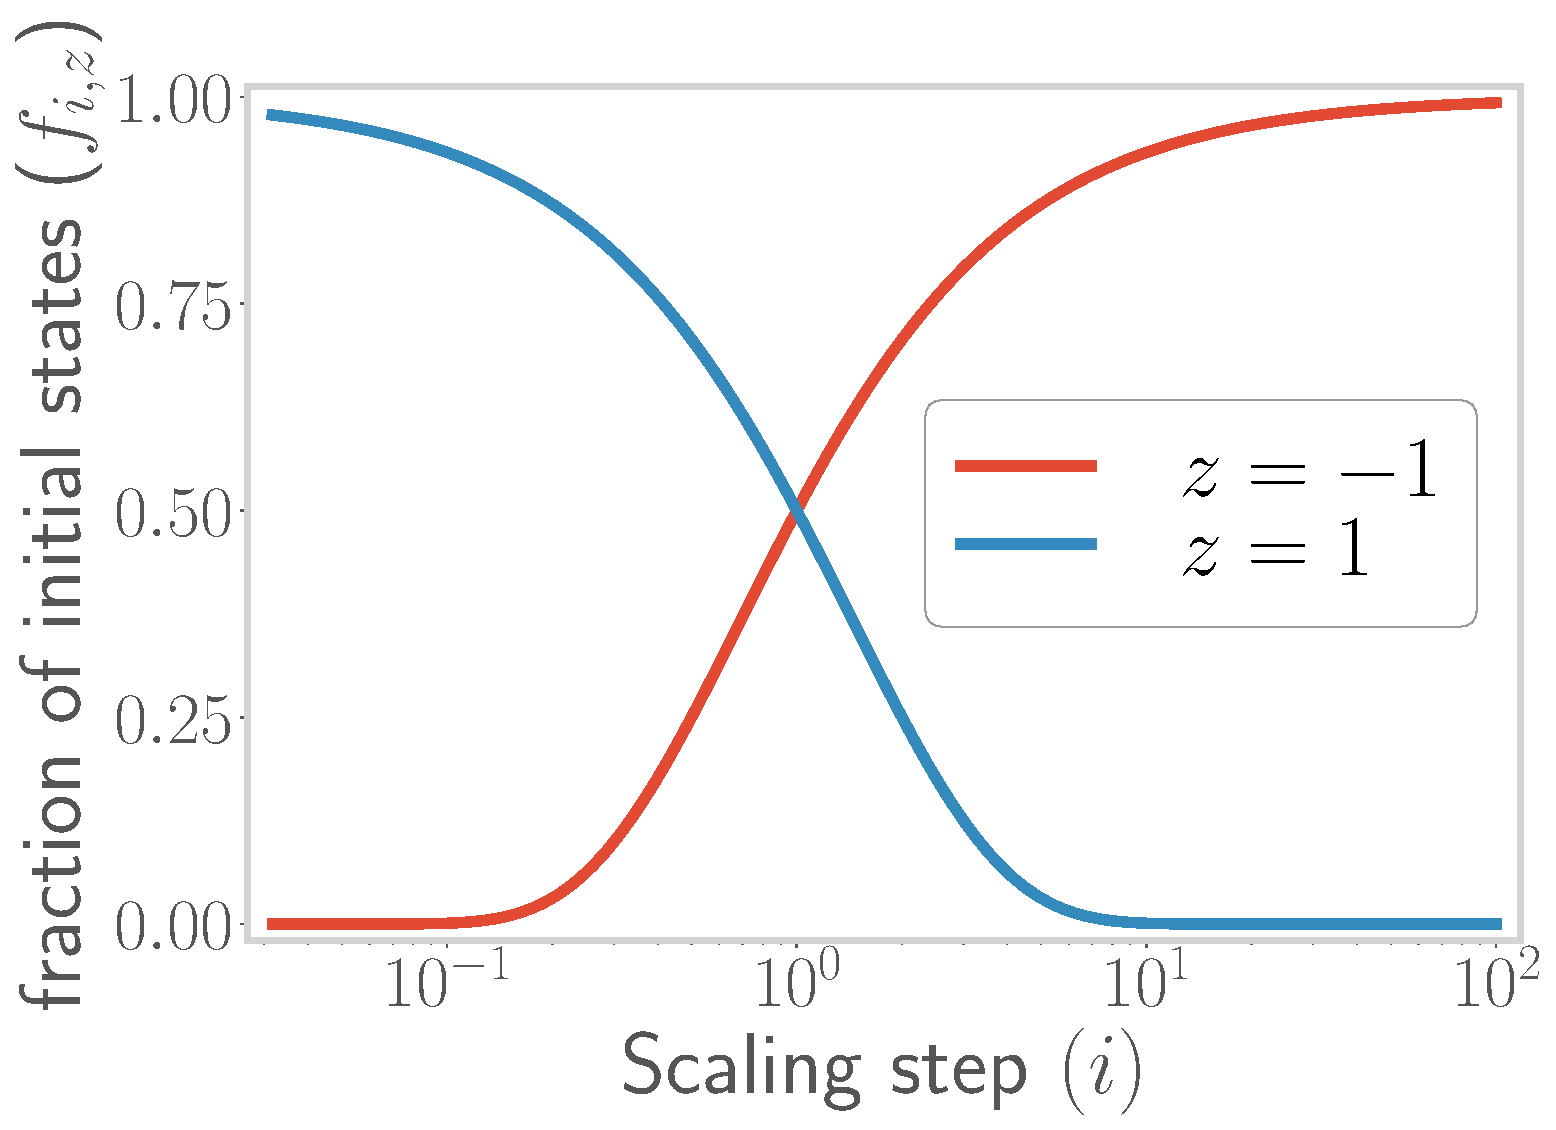
\includegraphics[width=0.5\textwidth]{figures/fraction.pdf}
\end{frame}


\begin{frame}{Simplest Limit}
\hspace*{\fill}
\begin{minipage}{0.5\textwidth}
Simplest case: \(j=0\)\\[5pt]
\begin{itemize}
	\item no coarse-graining or fine-graining\\[20pt]
	\item \(A_z(0) \longrightarrow ~ ~\)\alert{cylindrical section}
\end{itemize}
\end{minipage}
\hspace*{\fill}
\begin{minipage}{0.4\textwidth}
	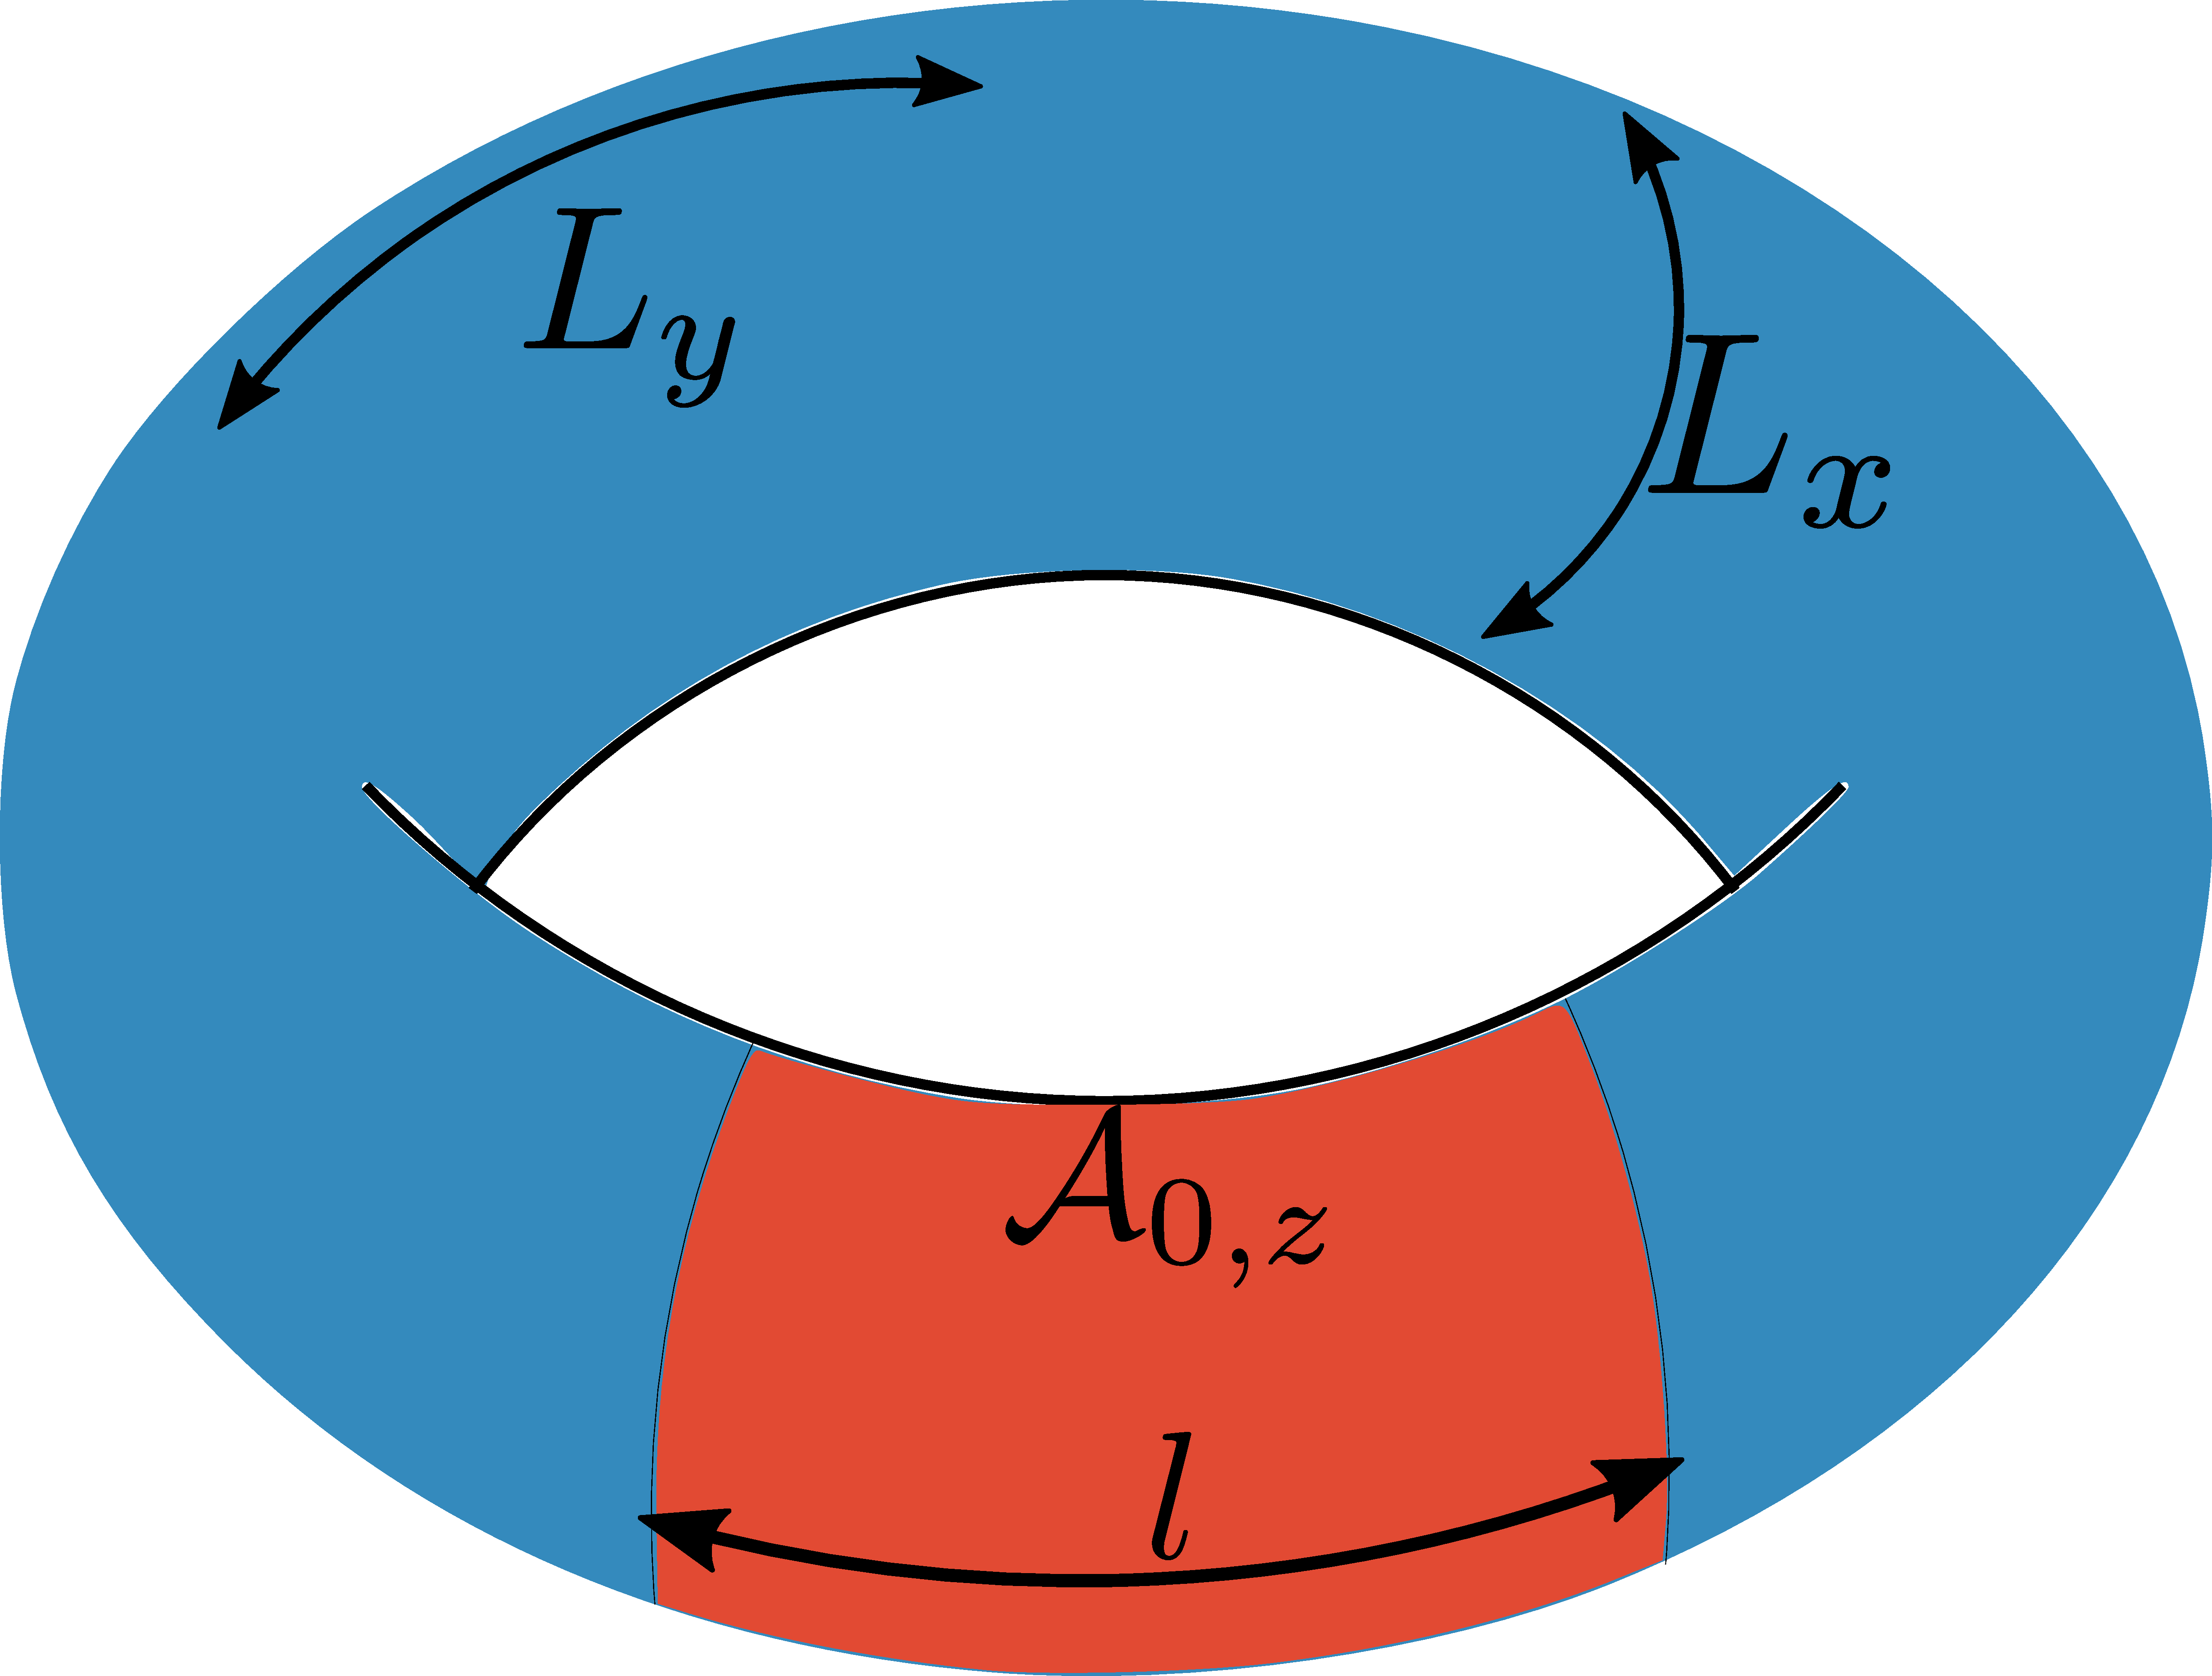
\includegraphics[width=0.8\textwidth]{figures/A_m1.pdf}
\end{minipage}

\vspace*{\fill}
\centering
In general:

\begin{minipage}{0.33\textwidth}
	\[\Delta n \sim \Delta k_x \sim 1/L_x ~ ~ ~\longrightarrow \]
\end{minipage}
\begin{minipage}{0.33\textwidth}
	\[ z > 0: \text{decreasing system size}\]
	\[ z < 0: \text{increasing system size}\]
\end{minipage}
\end{frame}

\begin{frame}{Subsystem Entanglement Entropy}
\footcite{Calabrese_2004,Casini_2005,Arias_2015,Chen_2017,Murciano_2020}
Modes are decoupled \(\longrightarrow\) entanglement is additive
\vspace*{\fill}
\[S_n(\phi) = c \log \left(\alpha L_x\right) - c \log |n + \phi|\]
\[S_{\mathcal{A}_z(j)} = \sum_{n \in \mathcal{A}_z(j)} S_n = f_z(j) c \alpha L_x - c \log \big|2\sin\left(\pi f_z(j)\phi\right)\big|\]
\[i < j, ~ ~ S_{i\cup j} =
	\begin{cases}
	S_{i}, ~ ~ z > 0\\
	S_{j}, ~ ~ z < 0
	\end{cases}
\]
\end{frame}

\begin{frame}{Entanglement Hierarchy}
\begin{minipage}{0.5\textwidth}
\[i < j, ~ ~ S_{i\cup j} =
	\begin{cases}
	S_{i}, ~ ~ z > 0\\
	S_{j}, ~ ~ z < 0
	\end{cases}
\]
\end{minipage}
\begin{minipage}{0.45\textwidth}
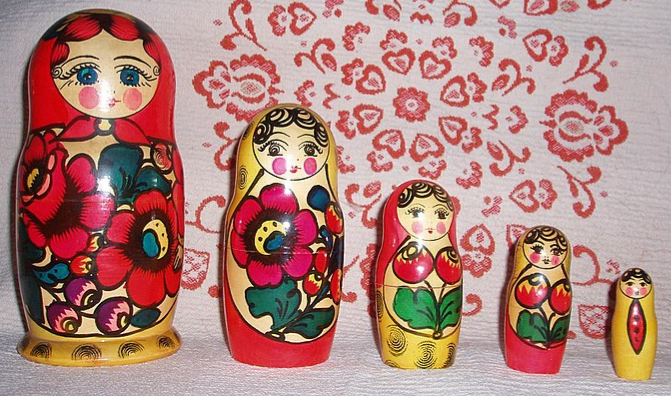
\includegraphics[height=0.3\textheight]{figures/Matroshka.png}
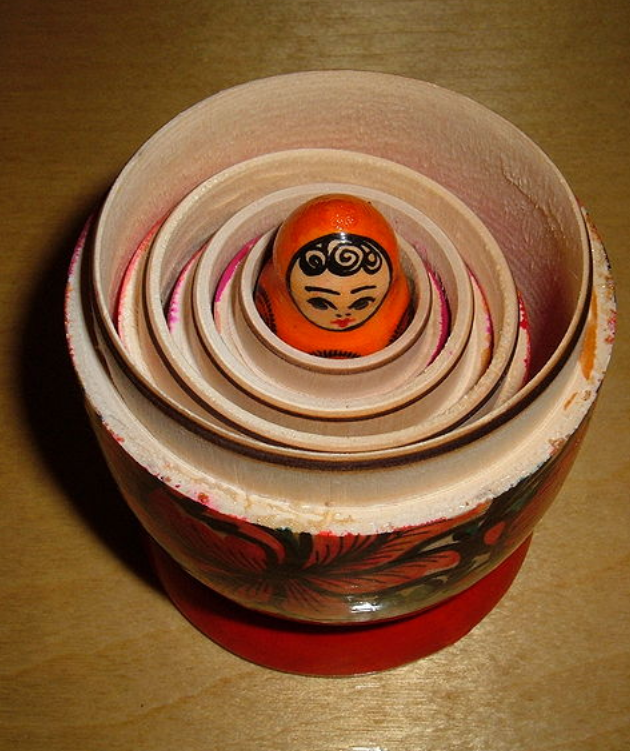
\includegraphics[height=0.3\textheight]{figures/nested.png}
\end{minipage}

\vspace*{\fill}

\begin{itemize}
	\item 
presents a \alert{hierarchy} of entanglement \(\longrightarrow\) EE distributed across RG steps:\\[10pt]
RG transformation \(\longrightarrow\) reveals entanglement

\vspace*{\fill}
\item distribution of entanglement also present in \alert{multipartite} entanglement:\\[10pt]
	mutual information and higher order measures, within one RG step or spread across the flow
\end{itemize}

\end{frame}

\section{Holographic Nature of the RG Flow}
\begin{frame}{Mutual Information = Distance}
\footcite{van2010building,lee2016,anirban_mott_2022}
	\alert{Mutual information}: ~ \(I^2(A:B) \equiv S(A) + S(B) - S(A \cup B)\) ~ ~ ~ (non-negative)\\[10pt]
	information gained about \(B\) upon measuring \(A\)\\[10pt]
	define distance along the RG: ~ ~ \(d_z(j) \equiv \log I^2_\text{max} - \log I_z^2(0:j) = \log t_z(j)\)

	\vspace*{\fill}

	\begin{minipage}{0.4\textwidth}
	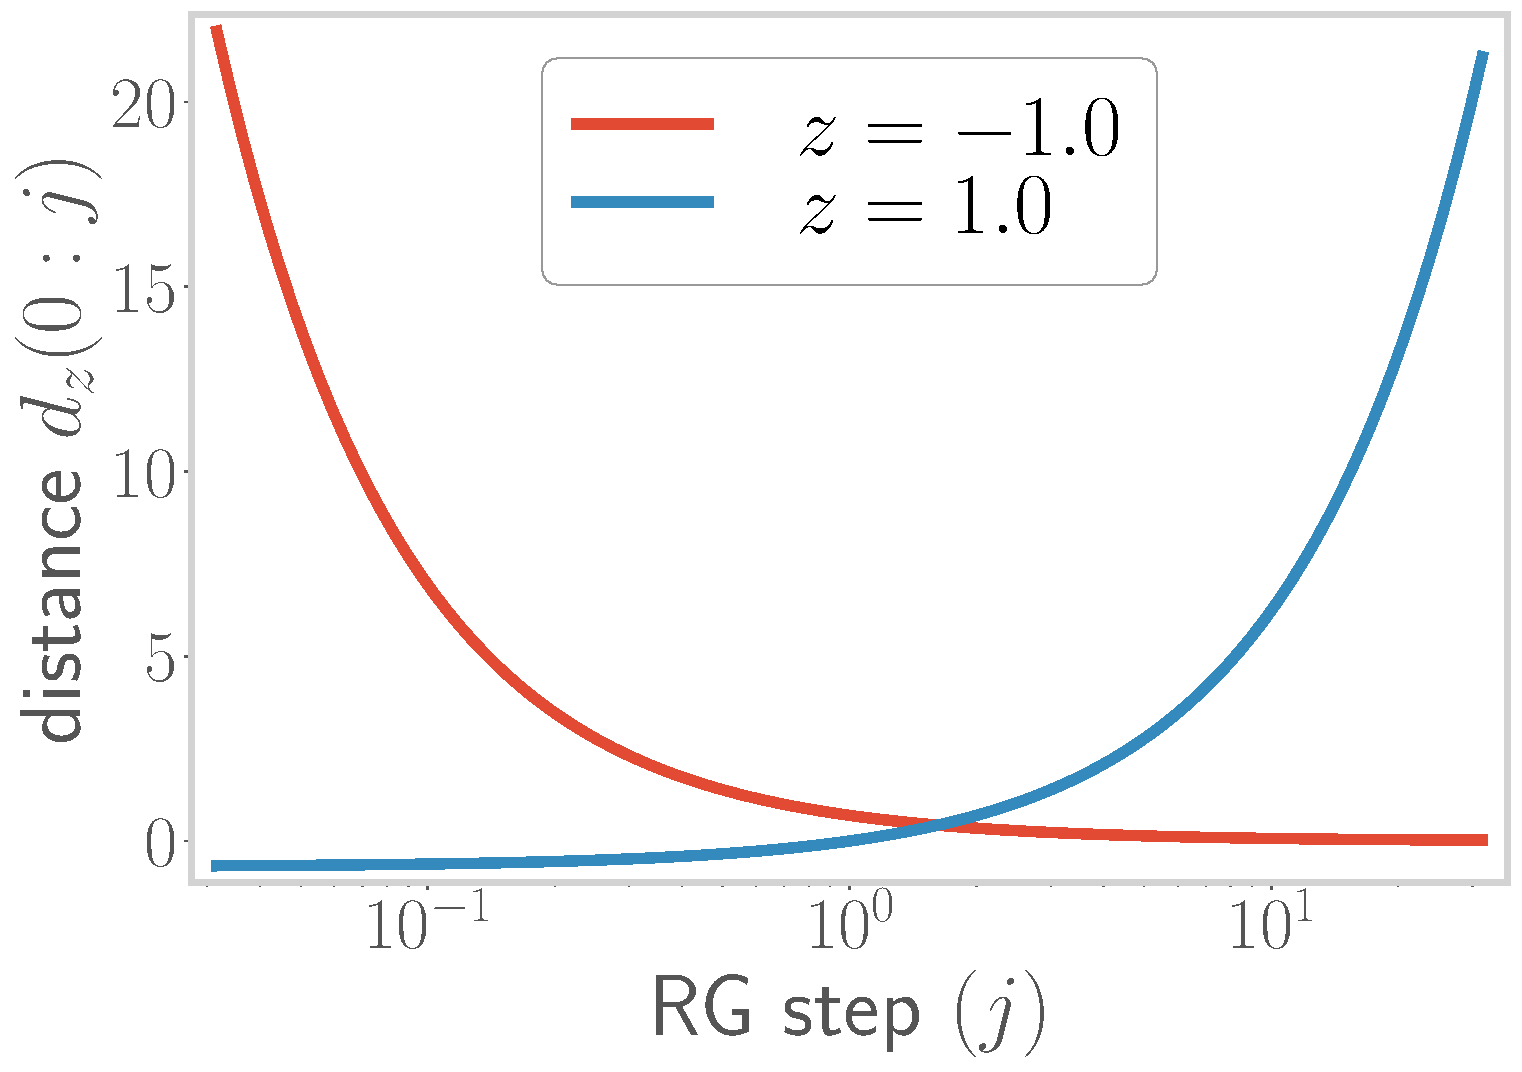
\includegraphics[width=\textwidth]{figures/distance1.pdf}
	\end{minipage}
	\hspace*{\fill}
	\begin{minipage}{0.55\textwidth}
		\centering
		For \(z > 0\):\\[5pt]
		\begin{itemize}
			\item mut. info. is maximum for small \(j\)\\[10pt]
			\item decreases for large \(j\)\\[10pt]
			\item corresponds to \alert{increasing distance}
		\end{itemize}
	\end{minipage}
\end{frame}

\begin{frame}{RG evolution = Emergent Distance}
	\footcite{lee2010,anirbanurg1,ryu2006,nozaki2012}
\only<1>{
	Define \(2-\)dimensional \(x-y\) structure\\[20pt]
	\begin{minipage}{0.5\textwidth}
	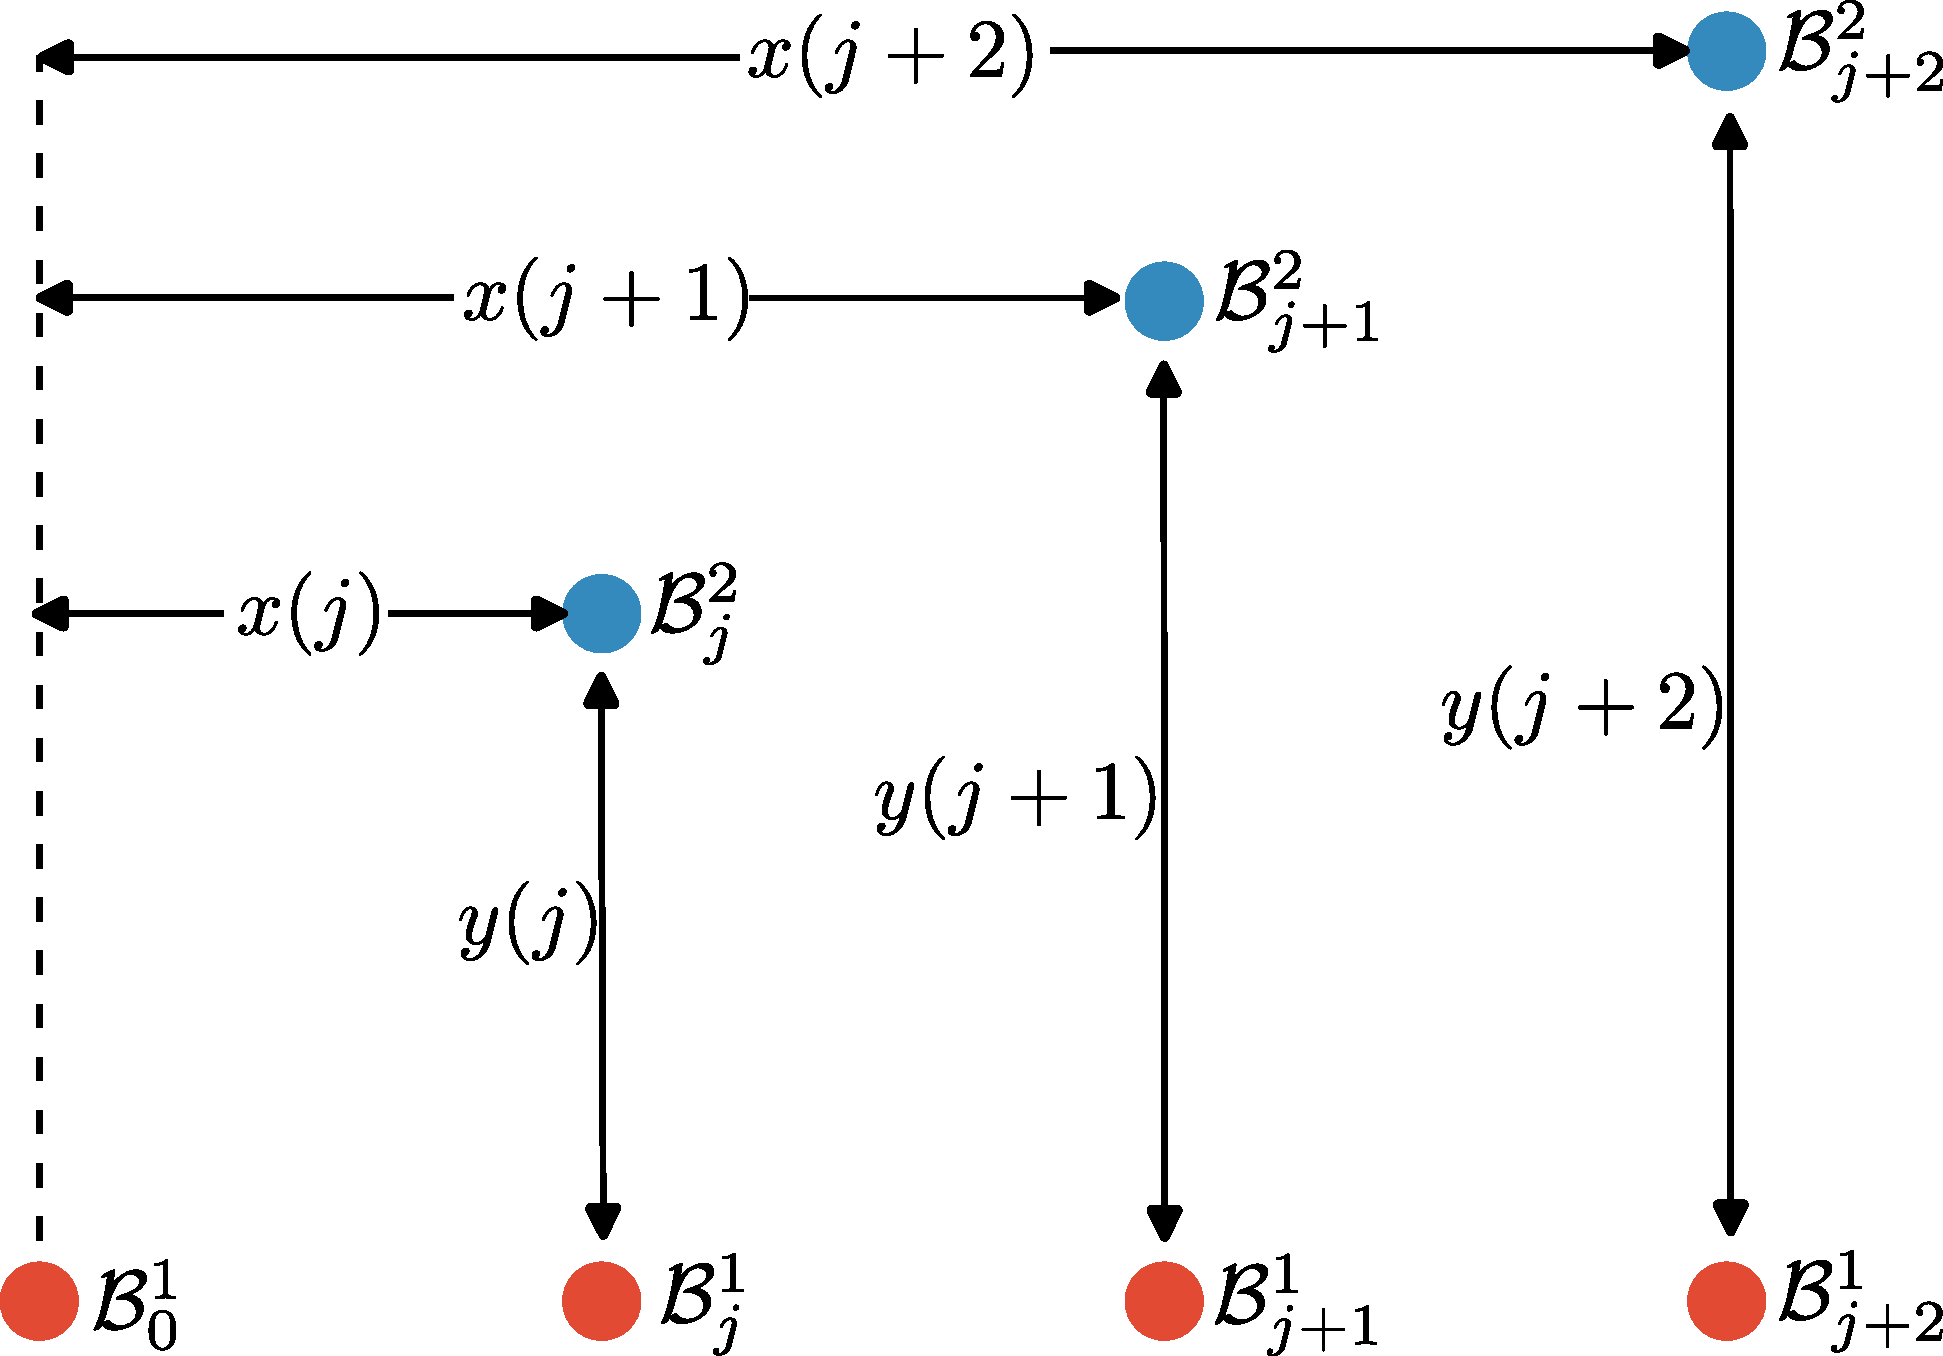
\includegraphics[width=\textwidth]{figures/curvature-scheme.pdf}
	\end{minipage}
	\hspace{\fill}
	\begin{minipage}{0.45\textwidth}
		\centering
	Red Circle: RG steps\\[10pt]
	Blue Circle: subsystems within an RG step
	\[x_z(j) = d_z(j) = \log t_z(j)\]
	\begin{equation*}\begin{aligned}
	y_z(j) = \log I^2_\text{max} - \log I_z^2(\mathcal{B}_j^1:\mathcal{B}_j^2) \\
	= \log t_z(j \pm 1)
	\end{aligned}\end{equation*}
	\end{minipage}
}
\only<2>{
	Define coupling that measures spectral gap:~ ~ \(g_z(j) = \log \frac{M_{n+1}(\phi) - M_n(\phi)}{2\pi/L_x} = \log t_z(j)\)\\[10pt]
	RG beta function for its evolution: ~ ~ \(\beta_z(j) = \Delta \log g_z(j) = z \log\left( 1 + j^{-1} \right) \)

	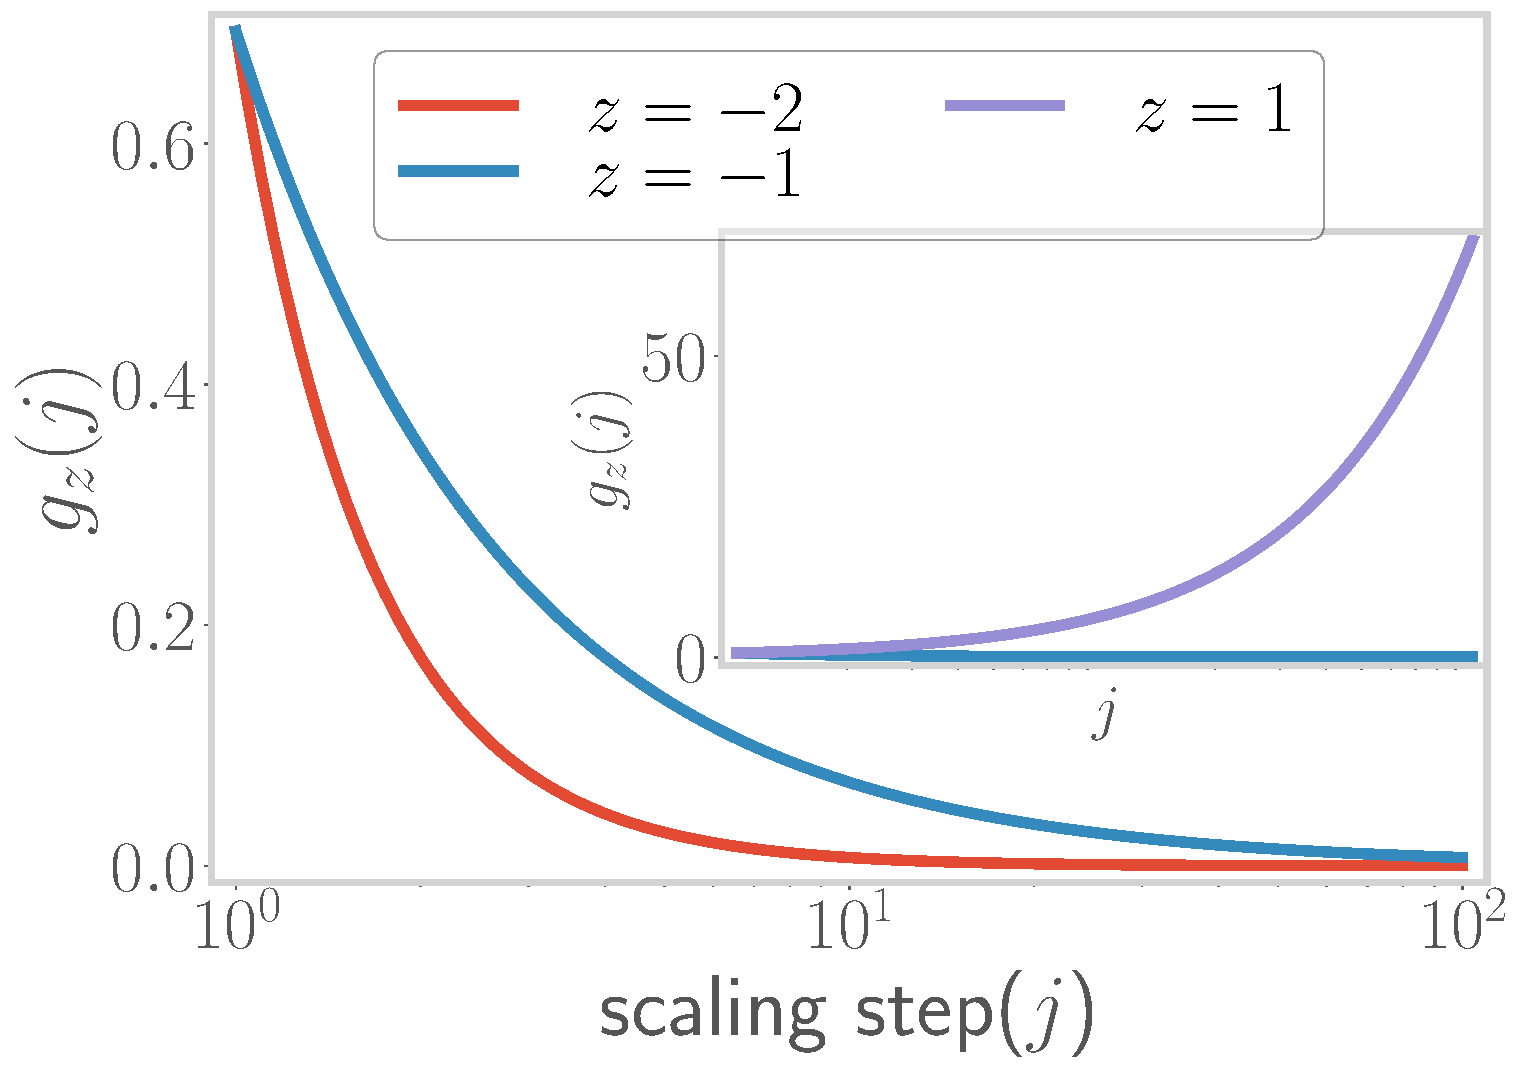
\includegraphics[width=0.45\textwidth]{figures/coupling.pdf}
	\hspace*{30pt}
	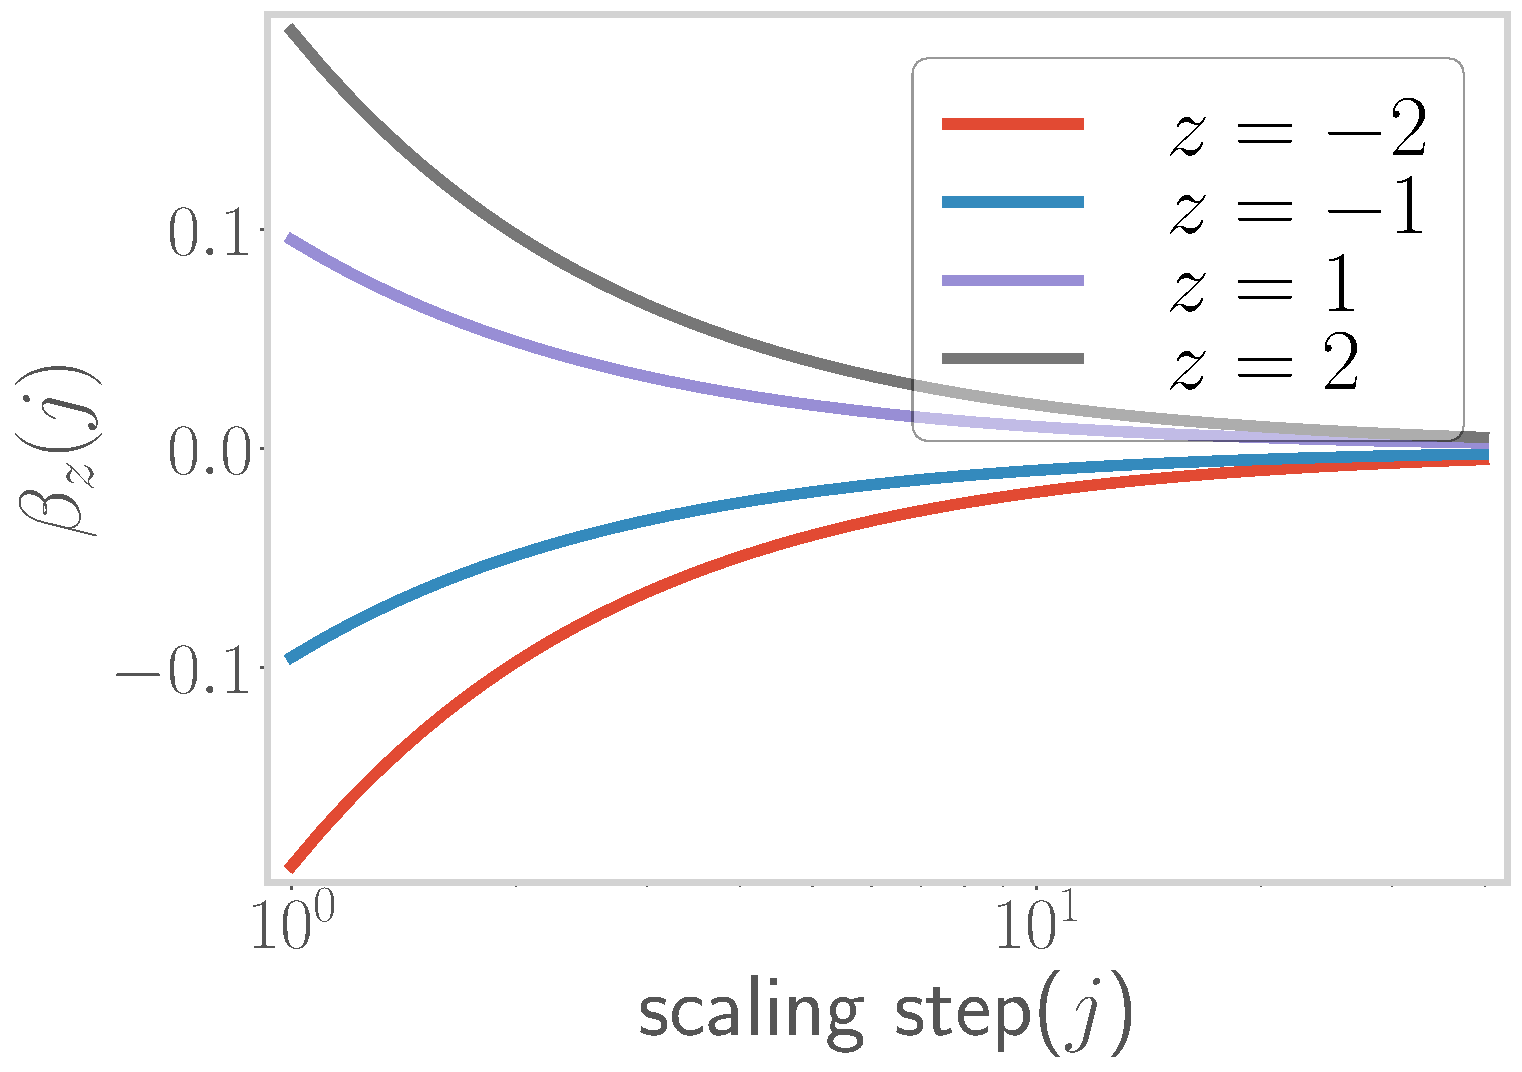
\includegraphics[width=0.45\textwidth]{figures/mass-beta.pdf}
}
\only<3>{
	RG beta function can be related to the \(x,y-\)distances
	\[x_z = \left( e^\frac{\beta_z}{z} - 1 \right)^{-z} \log 2\]
	\[y_z = \begin{cases}
		x_z e^\beta,~~ &z > 0\\
		x_z \left(2 - e^\frac{\beta}{z}\right)^z,~~ &z < 0\\
	\end{cases}\]
	\\[10pt]
	explicit relation between the RG flow and the emergent \alert{geometry}
}
\end{frame}

\begin{frame}{Curvature of Emergent Space}
	Define first and second derivatives in emergent space
	\[v_z(j) \equiv \frac{\Delta y_z(j)}{\Delta x_z(j)} =\begin{cases}
		\frac{\left(j+2\right)^z - \left(j+1\right)^z}{\left(j+1\right)^z - j^z},~ ~ z > 0\\
		\frac{\left(j\right)^z - \left(j-1\right)^z}{\left(j+1\right)^z - j^z},~ ~ z < 0\\
	\end{cases}
\]
\[
	v^\prime_z(j) \equiv \frac{v_z(j+1) - v_z(j)}{x_z(j+1) - x_z(j)}
\]
Define curvature using them: {\(\kappa_{z}(j) = \frac{v^\prime_z(j)}{\left[1 + v_z(j)^2\right]^\frac{3}{2}}\)}\\[10pt]
\(\longrightarrow\) can be expressed in terms of \(\beta_z(j)\)
\end{frame}

\begin{frame}{Curvature of Emergent Space}
\begin{minipage}{0.45\textwidth}
	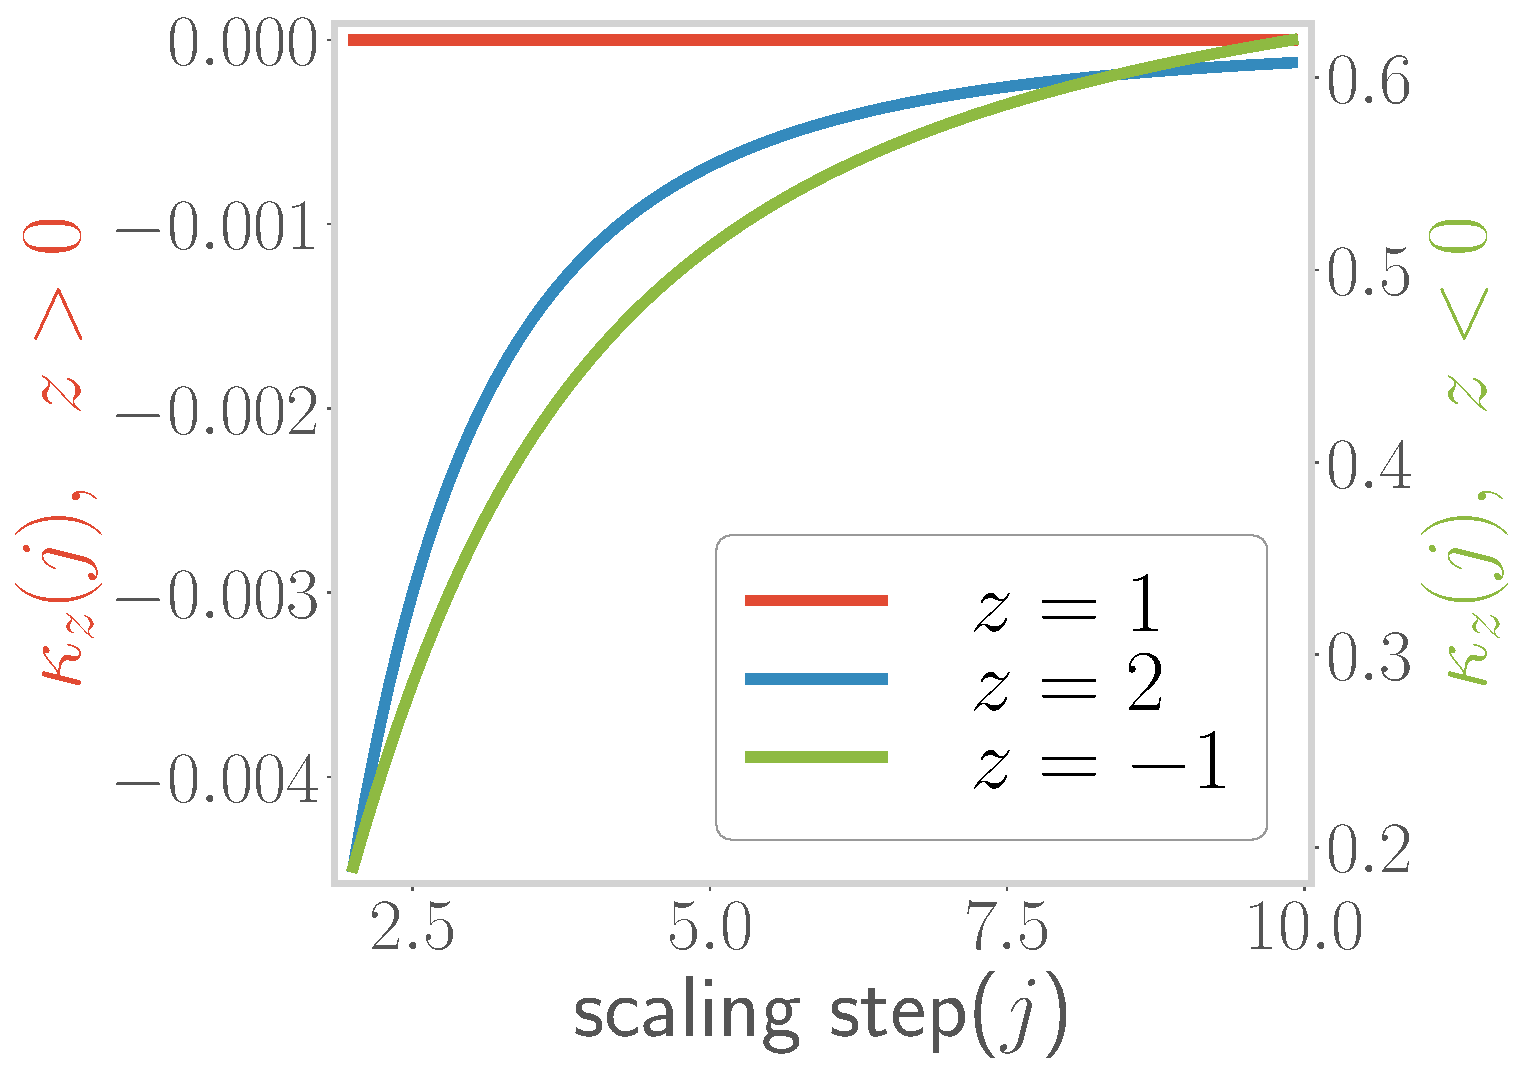
\includegraphics[width=\textwidth]{figures/curvature-pos.pdf}
\end{minipage}
\begin{minipage}{0.5\textwidth}
	\begin{itemize}
		\item positive curvature for \(z < 0\)\\[10pt]
		\item zero curvature for \(z = 1\)\\[10pt]
		\item negative curvature for \(z  > 1\)\\[10pt]
		\item \alert{asymptotically flat} for large \(j\), at all \(z\)
	\end{itemize}
\end{minipage}

\end{frame}

\begin{frame}{The Sign of Curvature is Topological!}
\only<1>{
	\[\gamma_z(j) \equiv 1 - v_z(j+1)/v_z(j), ~ ~ ~\alpha_z(j) = y_z(j+1) - y_z(j)\]

\vspace*{\fill}

	\[\kappa_{z}(j) = -\frac{\alpha_z(j)~\gamma_z(j)}{\left(\Delta x_z(j)\right)^2\left[1 + v_z(j)^2\right]^\frac{3}{2}} \implies \text{sign}\left[\kappa_z(j)\right] = -\text{sign}\left[\alpha_z(j)\right]\text{sign}\left[\gamma_z(j)\right]\]

\vspace*{\fill}
\[
	\text{sign}\left[\kappa_z\right] = \begin{cases}
		-1 ,~ ~ z \geq 1\\
		1 ,~ ~ ~ ~ z \leq -1\\
	\end{cases} = ~ ~ \begin{cases}
		-\text{sign}\left[\gamma_z(j)\right] ,~ ~ z \geq 1\\
		-\text{sign}\left[\alpha_z(j)\right] ,~ ~ z \leq -1\\
	\end{cases}
\]

}
\only<2>{
\begin{minipage}{0.49\textwidth}
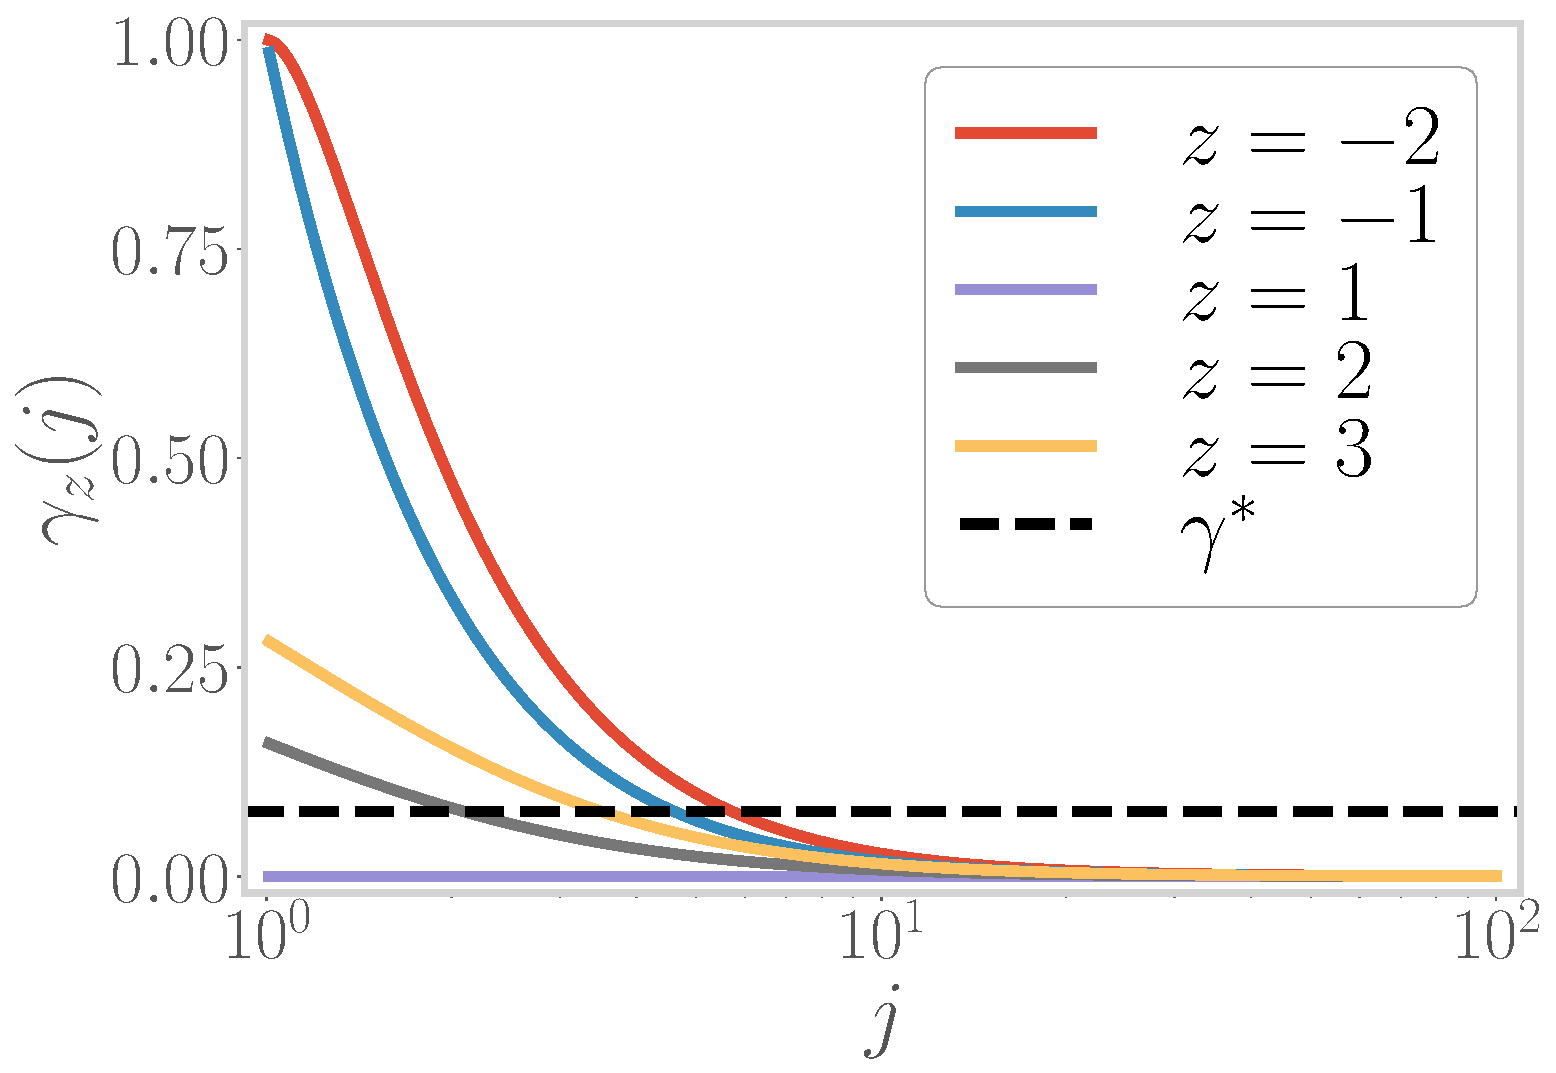
\includegraphics[width=0.9\textwidth]{figures/gamma.pdf}
\end{minipage}
\begin{minipage}{0.49\textwidth}
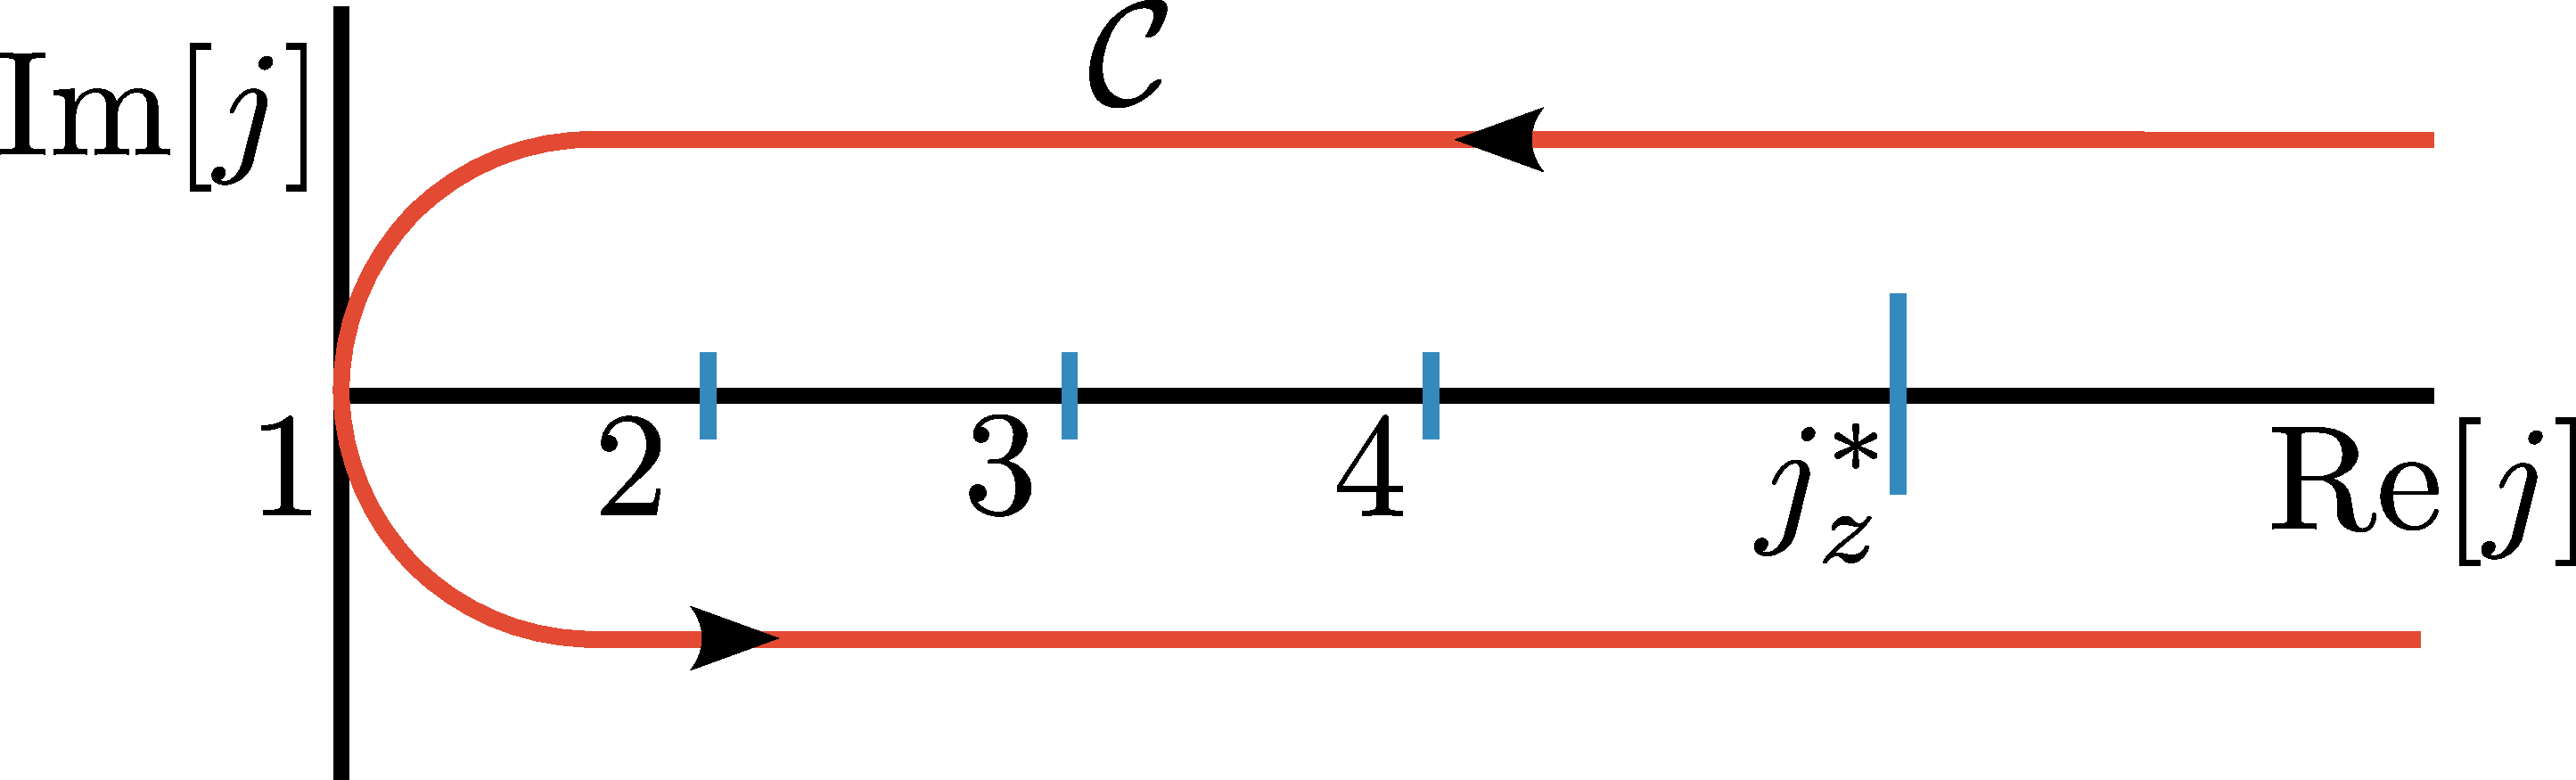
\includegraphics[width=0.9\textwidth]{figures/curvature-contour.pdf}
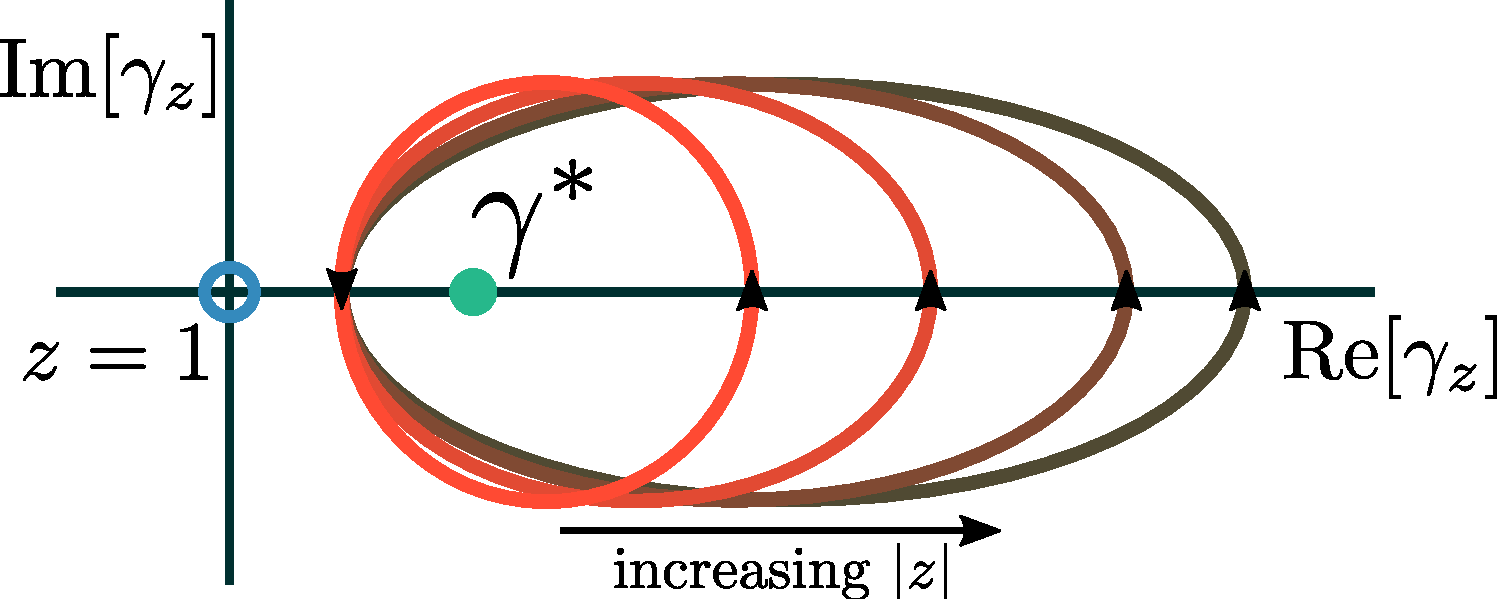
\includegraphics[width=0.9\textwidth]{figures/curvature-winding.pdf}
\end{minipage}\\[10pt]

\begin{itemize}
	\item \(\ln \left(\gamma - \gamma^*\right)\) has branch point at \(\gamma^*\), can be avoided for \(z=1\), \alert{contour is trivial}\\[10pt]
	\item cannot be avoided for \(z \neq 1\) \(\longrightarrow\) presence of \alert{singularity} \(\longrightarrow\) encoded through \alert{winding number}
\end{itemize}


}
\only<3>{
\begin{minipage}{0.5\textwidth}
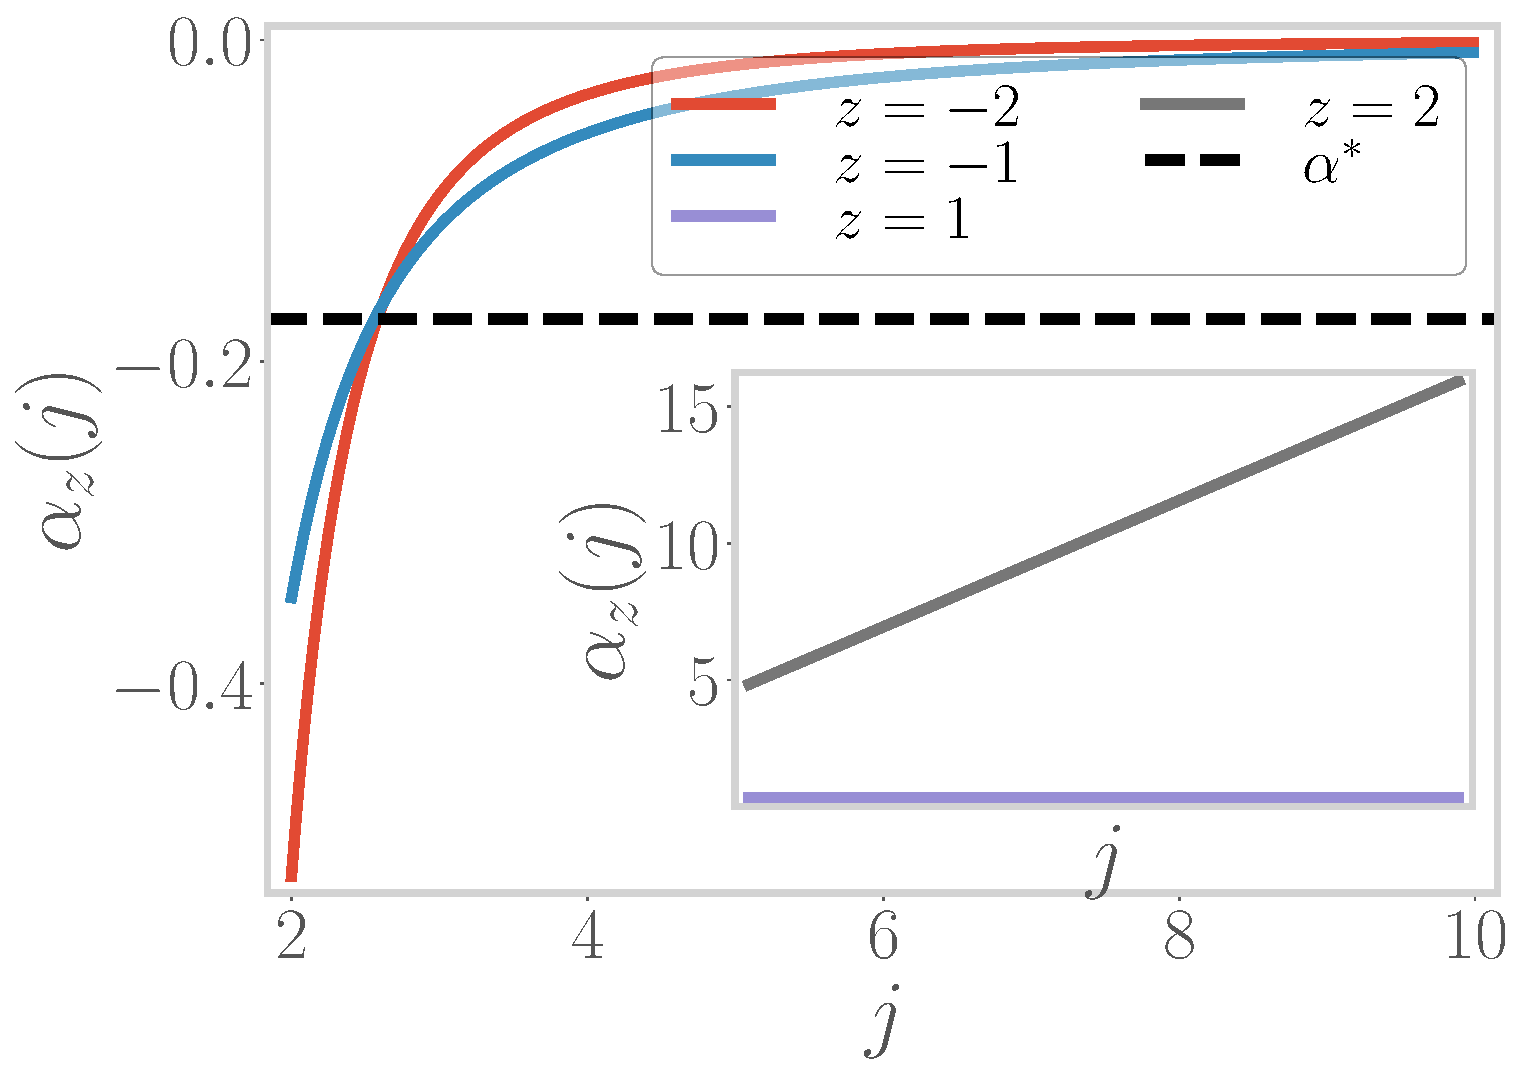
\includegraphics[width=0.8\textwidth]{figures/alpha.pdf}

\vspace{\fill}
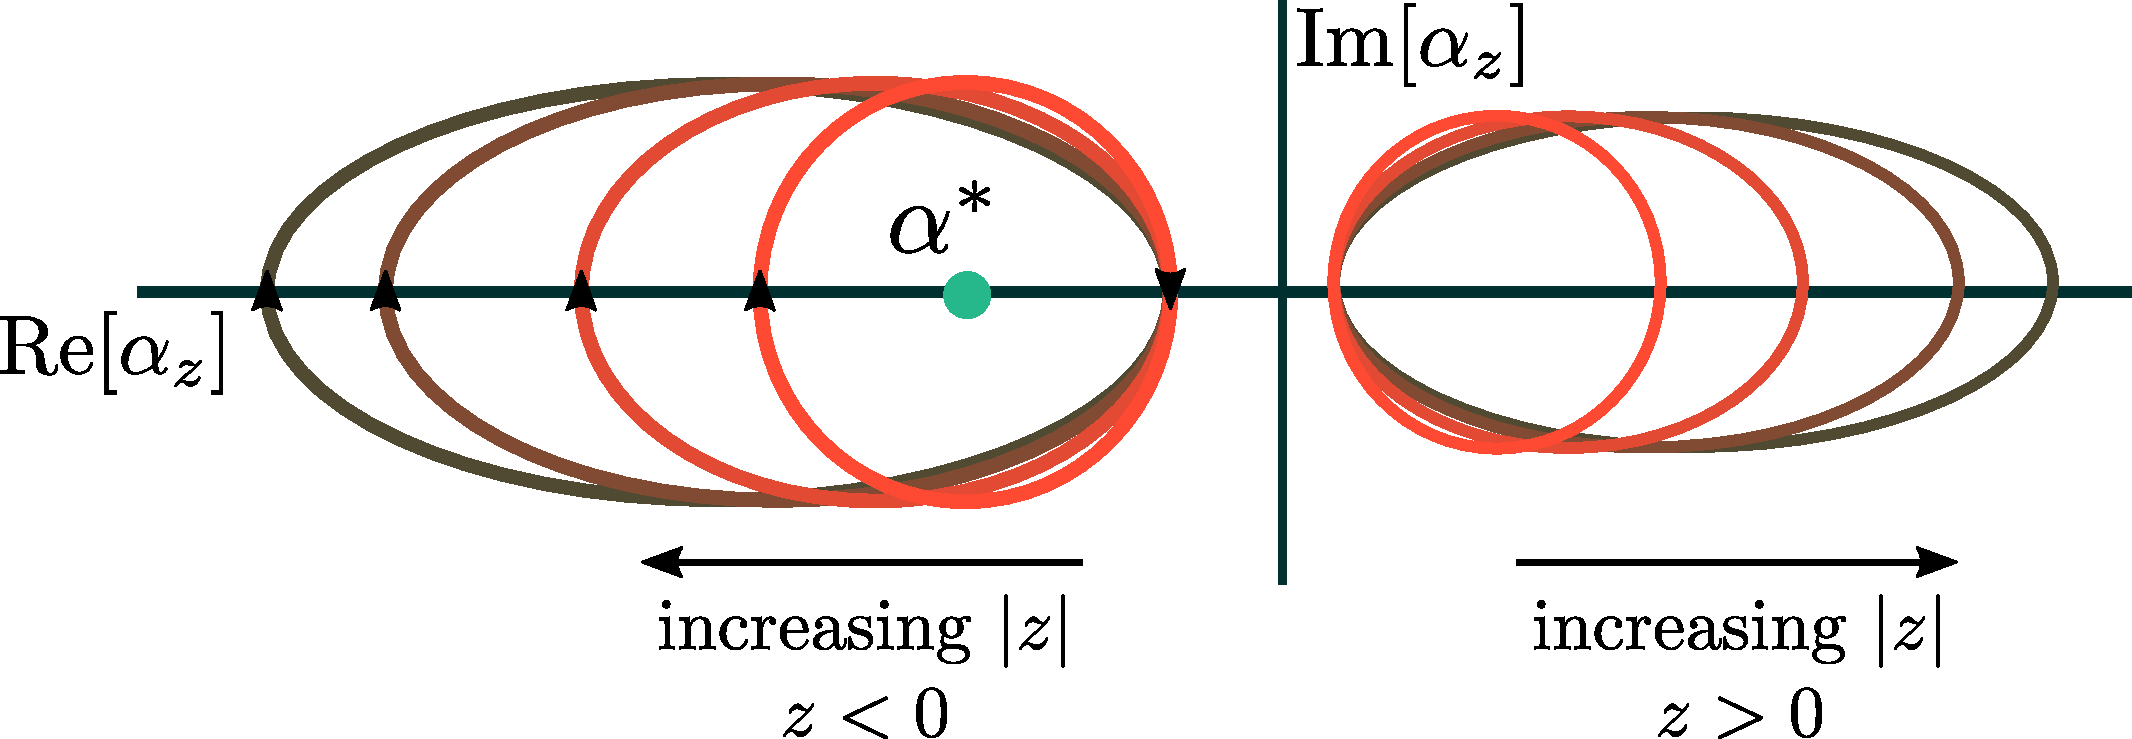
\includegraphics[width=\textwidth]{figures/alpha-winding.pdf}
\end{minipage}
\begin{minipage}{0.45\textwidth}
	very similar thing holds for \(\alpha_z\)
	\begin{itemize}
		\item singularity exists only for \(z < 0\)
		\item otherwise contour can be trivialised\\[20pt]
	\end{itemize}
	

	Curvature can be written as the product of \alert{winding numbers}:
	\[\text{sign}\left[\kappa_z\right] = \mathcal{W}_z\left( \gamma^* \right) \times \left[2\mathcal{W}^\prime_z\left( \alpha^* \right) - 1\right] \]
	Winding numbers count singularities, robust against deformations
\end{minipage}

}
\only<4>{

	{\bf Significance of change in topology}
	\begin{itemize}
		\item sign of \(z\) reflects the RG relevance/irrelevance of \(g_z\) in the microscopic fermionic theory
		\item change in sign of \(z\) is hence a \alert{phase transition} in the microscopic theory that changes the topology of the Fermi surface
	\end{itemize}

}
\end{frame}

\section{Entanglement Holography and Fermionic Criticality}
\begin{frame}{Critical Fermi Surface = Wormhole Geometry}
	\only<1>{
	\footcite{anirbanurg1,Heath_2020}
	Between \(z < 0\) and \(z > 0\), two \alert{topological transitions} occur:
	\begin{itemize}
		\item Curvature changes sign
		\item Fermi surface becomes gapped \(\rightarrow\) change in Luttinger's volume
		\item Reflects a phase transition in the underlying interacting fermionic theory
	\end{itemize}
	\vspace{\fill}
	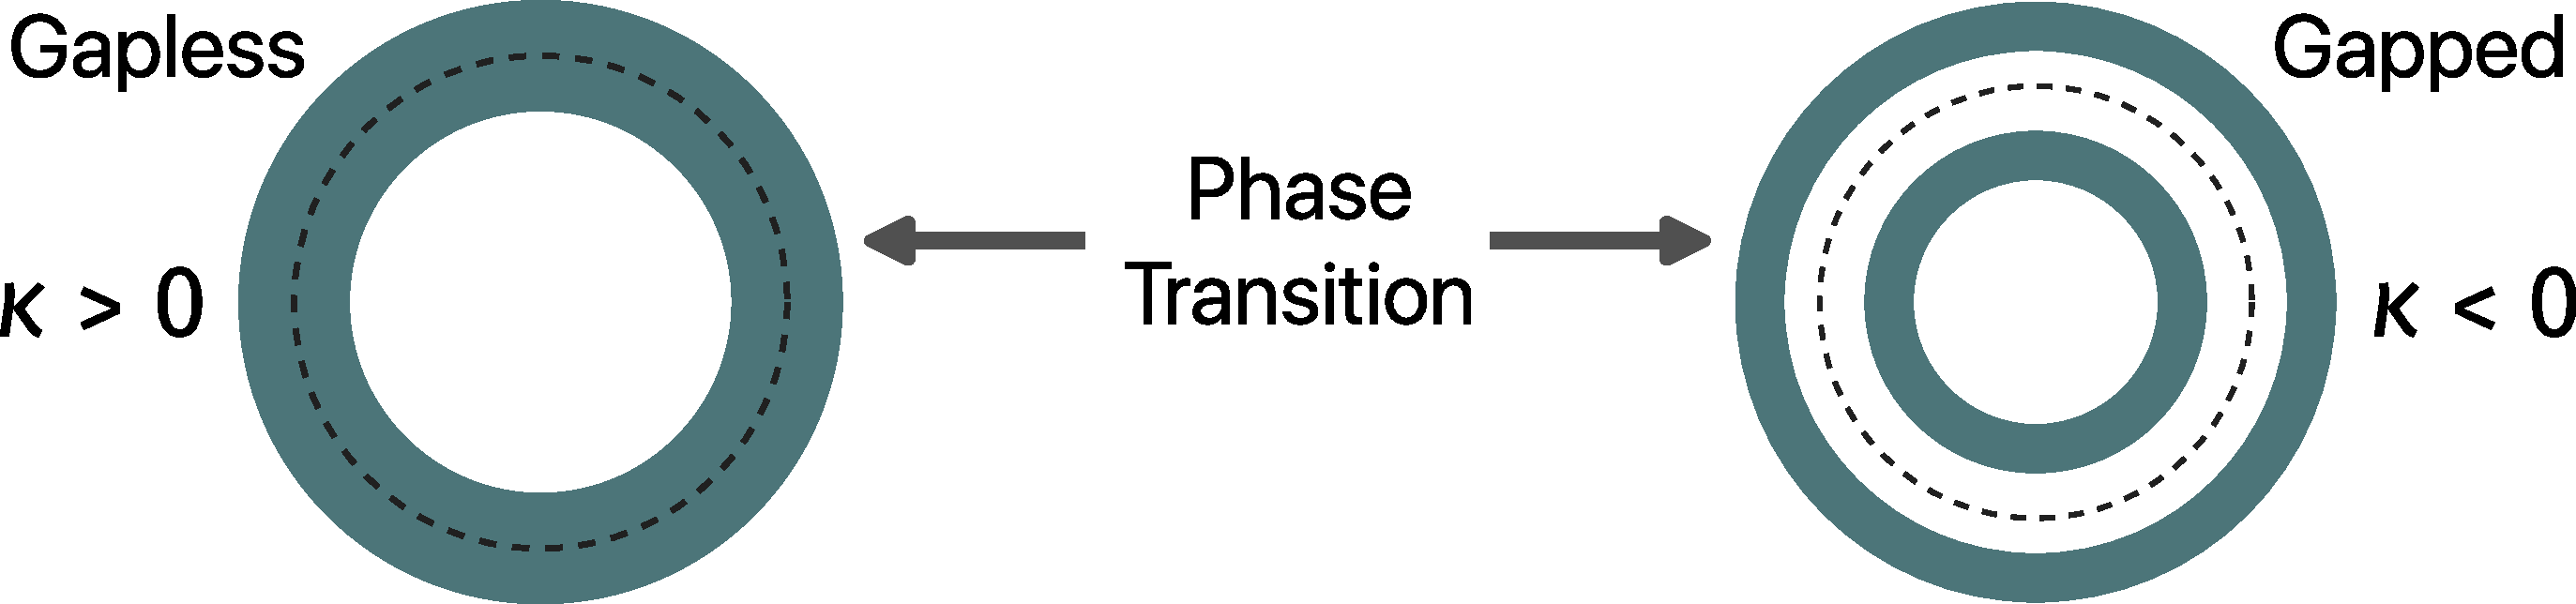
\includegraphics[width=0.9\textwidth]{figures/fermionicTransition.pdf}
}
\only<2>{
	\footcite{van2010building,cao2017}
	Also involves transition in nature of UV-IR entanglement
	\begin{itemize}
		\item Finite entanglement between UV and IR for \(z < 0\) (\alert{connected spaces})
		\item Vanishing entanglement between UV and IR for \(z > 0\) (\alert{disconnected spaces})\\[10pt]
	\end{itemize}
	At transition, minimal entanglement between two \\
	almost disconnected spaces \(\rightarrow\) \alert{wormhole geometry}!\\[10pt]

	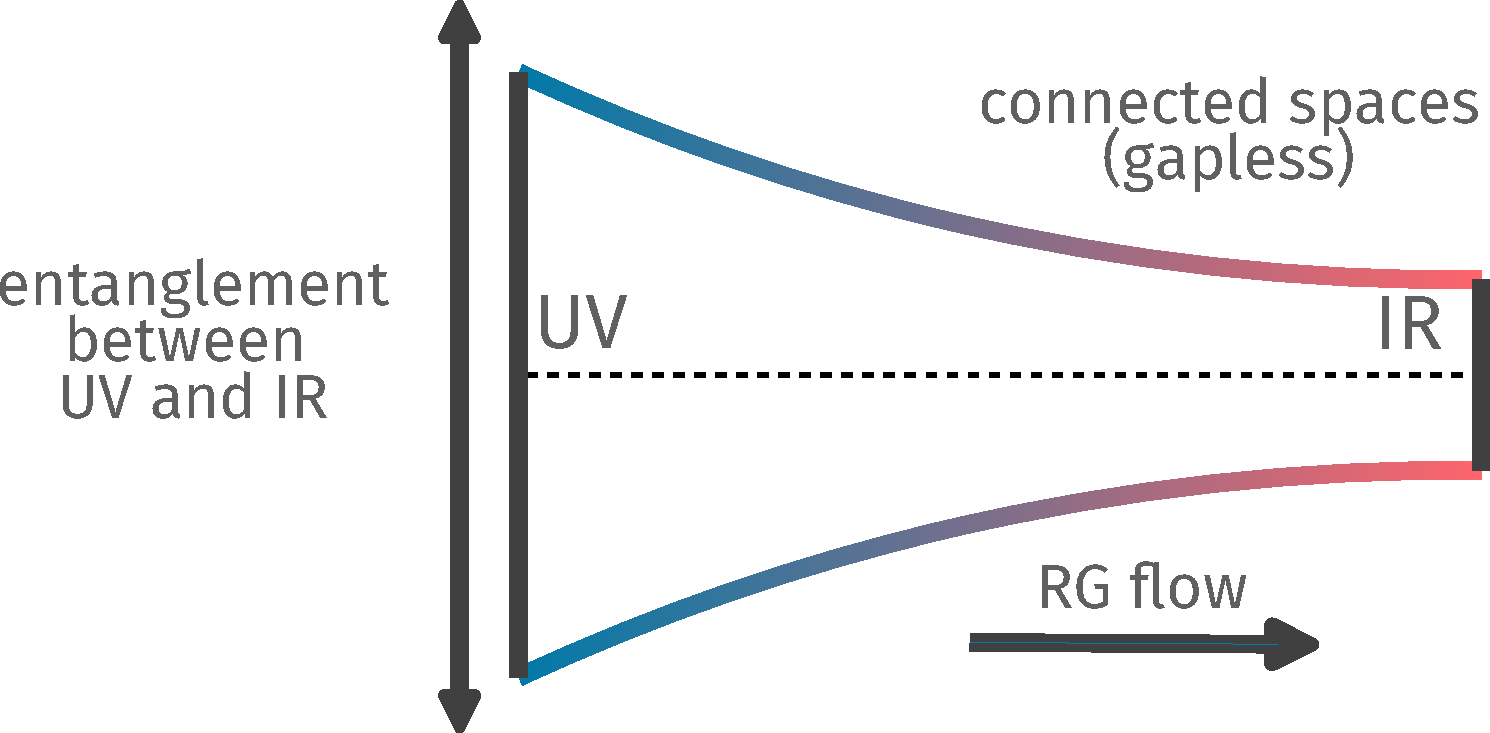
\includegraphics[width=0.4\textwidth]{figures/wormhole_gapless.pdf}
	\hspace{\fill}
	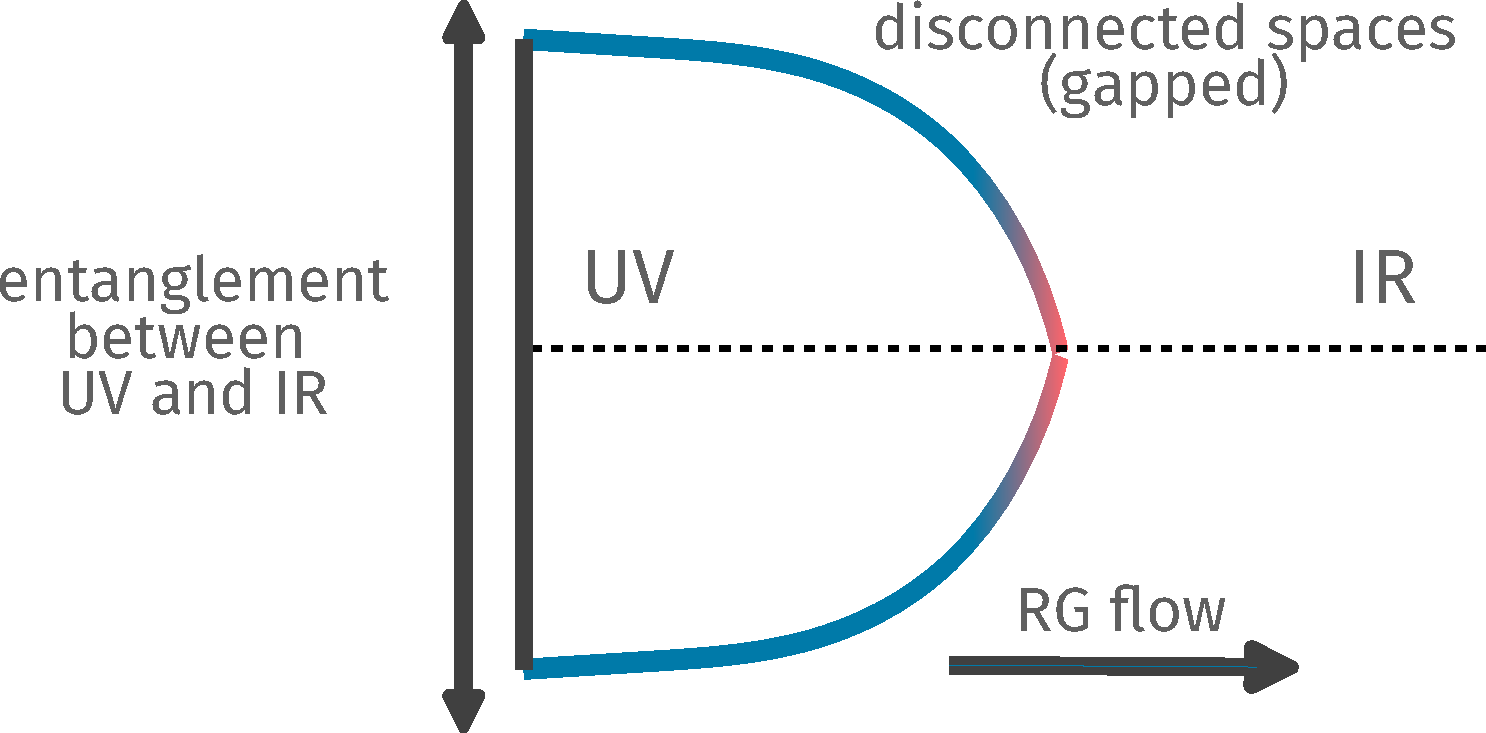
\includegraphics[width=0.4\textwidth]{figures/wormhole_gapped.pdf}
}
\end{frame}

\section{Topological Content of Entanglement}
\begin{frame}{Luttinger Volume and Flux-Dependent Entanglement}
	\only<1>{
	\footcite{oshikawa2000topological}
	Spectral flow: \(k_n = 2\pi n/L_x,\quad n \to n + \phi(\mathrm{flux})\)
	\begin{itemize}
		\item Tuning flux by one unit removes one \(k-\)state from Fermi volume
		\item Fermi momentum is therefore linked to the maximum flux \(\phi^*\)
	\end{itemize}

	\vspace{\fill}
	No. of states within Fermi volume = number of integers between \(0^+\) and \({\phi^*}^+\).

	\vspace{\fill}
	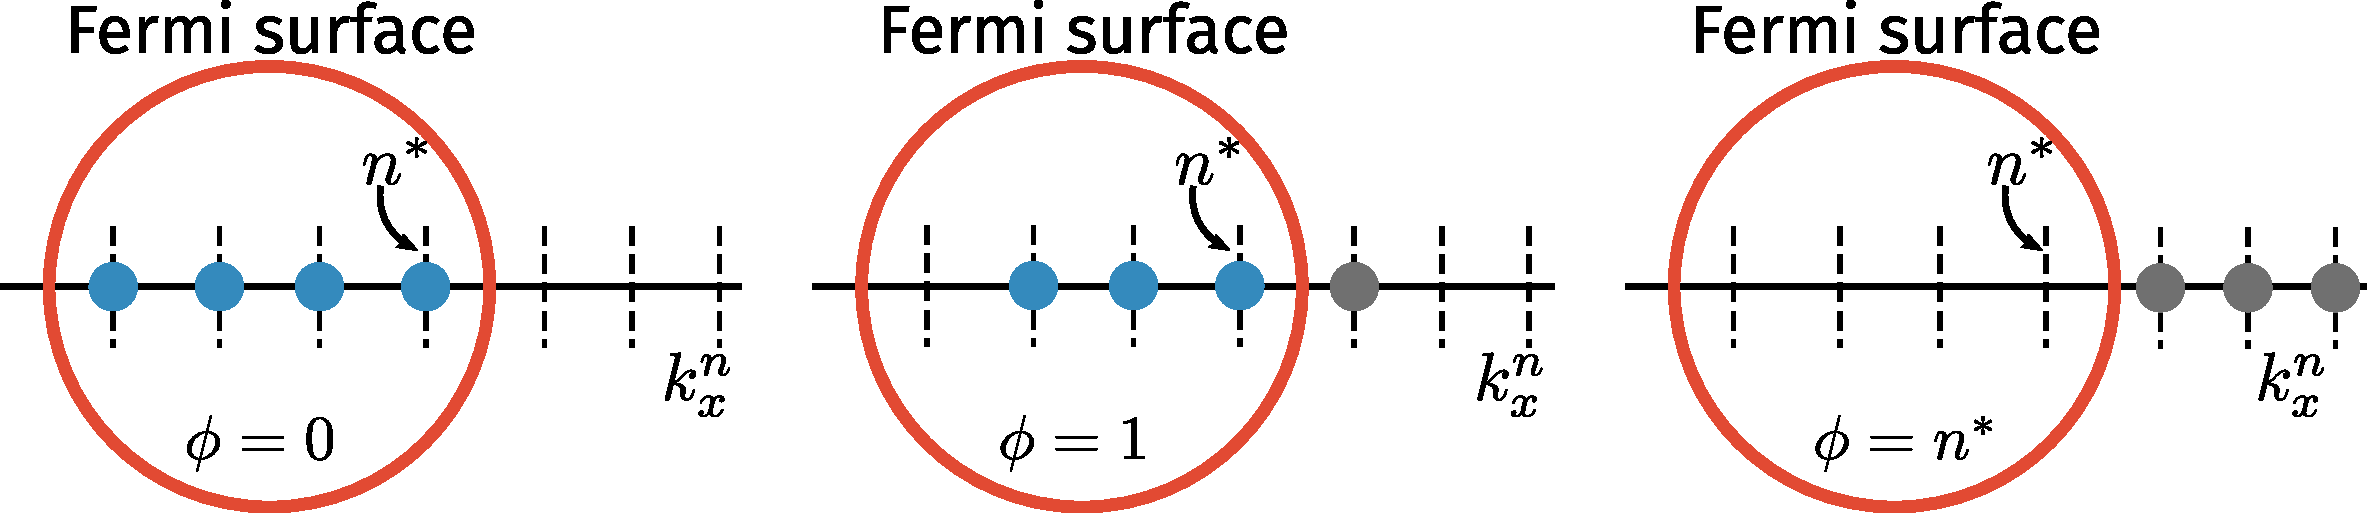
\includegraphics[width=0.8\textwidth]{figures/spectral-flow.pdf}
}
\only<2>{
	Consider function \(Q(\phi) = f\left[\frac{1}{\sqrt 2} - |\sin \pi \phi f|\right]\)\\[10pt]
	Goes through zero twice when \(\phi f\) changes by one unit: \(\phi f = 1/4, 3/4\)\\[10pt]
	\vspace{\fill}
	\begin{minipage}{0.4\textwidth}
	Fermi volume = no. of poles of \(Q^{-1}\)\\
	(residue $\propto$ no. of poles): 
	\[\sim \frac{1}{2}\oint_{\mathcal{C}} \frac{d\phi}{Q(\phi)} \sim \oint_{Y(\mathcal{C})} \frac{dY}{Y}\]
	Integral is \alert{quantised}!
	\end{minipage}
	\hspace*{\fill}
	\begin{minipage}{0.58\textwidth}
		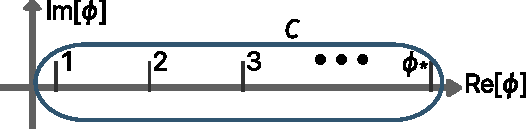
\includegraphics[width=\textwidth]{figures/contour.pdf}
	\end{minipage}
	\[Y = r e^{i\theta} \implies W = \oint_{Y(\mathcal{C})} \frac{dY}{Y} \sim \oint~d\theta = 0, 2\pi, 4\pi ,\ldots\]
}
\only<3>{
	\footcite{oshikawa2000topological,seki2017topological}
	\begin{minipage}{0.5\textwidth}
	\begin{itemize}
		\item Fermi volume is the \alert{winding number} of \(Y(C)\) around \(Y=0\)\\
		\item Topological in nature: Invariant under small deformations of the contour \(C\)
	\end{itemize}
	\end{minipage}
	\hspace*{\fill}
	\begin{minipage}{0.48\textwidth}
		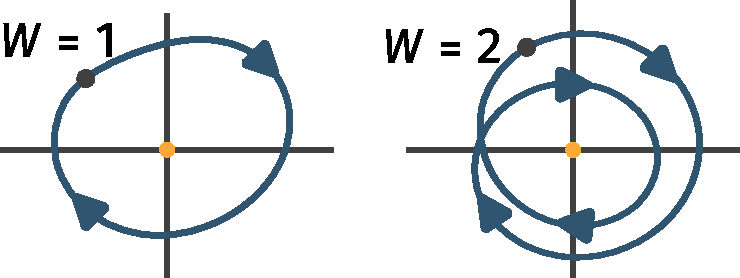
\includegraphics[width=\textwidth]{figures/windingNumber.pdf}
	\end{minipage}

	\flushleft
	\alert{Key points}
	\begin{itemize}
		\item Topological content of entanglement is the link to LV via spectral flow
		\item Yet another route to visualising LV as a topological invariant
		\item \alert{Boundary conditions} are important: No entanglement flow in localised states
	\end{itemize}
}
\end{frame}

\section{Concluding Remarks}
\begin{frame}{Summary of Results}
	\begin{itemize}
		\item Entanglement renormalisation = emergent distance scale. \\[10pt]
		\item Nature of emergent space depends on anomalous dimension of RG flow.\\[10pt]
		\item Change in curvature corresponds to fermionic phase transition and a wormhole geometry.\\[10pt]
		\item Topological structure of entanglement spectrum determines LV.\\[10pt]
	\end{itemize}
\end{frame}

\begin{frame}{Some Results I Didn't Have The Patience to Build Slides For}
	(\alert{But then I felt bad so I added this slide.})

	\begin{itemize}
		\item We can construct a `discrete metric' for our emergent dimension, by calculating the minimum distance between two points (geodesics).
		\item Such a metric can be related to the stress-energy tensor of the CFT, which takes us closer to Einstein-like field equations.
		\item We can define an expansion parameter (change of area of RG trajectories) that relates to the curvature, leading to equations similar to Raychaudhuri equation.
		\item Exploring the entanglement for a gapped system with a magnetic field (QHE) allows us to relate the topology of the entanglement to the Chern number.
	\end{itemize}

\end{frame}

\begin{frame}{}
	\LARGE Thank you!
\end{frame}
\printbibliography

\end{document}
